\iffalse
This file is protected by Copyright. Please refer to the COPYRIGHT file
distributed with this source distribution.

This file is part of OpenCPI <http://www.opencpi.org>

OpenCPI is free software: you can redistribute it and/or modify it under the
terms of the GNU Lesser General Public License as published by the Free Software
Foundation, either version 3 of the License, or (at your option) any later
version.

OpenCPI is distributed in the hope that it will be useful, but WITHOUT ANY
WARRANTY; without even the implied warranty of MERCHANTABILITY or FITNESS FOR A
PARTICULAR PURPOSE. See the GNU Lesser General Public License for more details.

You should have received a copy of the GNU Lesser General Public License along
with this program. If not, see <http://www.gnu.org/licenses/>.
\fi

%----------------------------------------------------------------------------------------
% Update the docTitle and docVersion per document
%----------------------------------------------------------------------------------------
\def\docTitle{OpenCPI\\ FSK App Guide}
\def\docVersion{1.3}
%----------------------------------------------------------------------------------------
\documentclass{article}
\iffalse
This file is protected by Copyright. Please refer to the COPYRIGHT file
distributed with this source distribution.

This file is part of OpenCPI <http://www.opencpi.org>

OpenCPI is free software: you can redistribute it and/or modify it under the
terms of the GNU Lesser General Public License as published by the Free Software
Foundation, either version 3 of the License, or (at your option) any later
version.

OpenCPI is distributed in the hope that it will be useful, but WITHOUT ANY
WARRANTY; without even the implied warranty of MERCHANTABILITY or FITNESS FOR A
PARTICULAR PURPOSE. See the GNU Lesser General Public License for more details.

You should have received a copy of the GNU Lesser General Public License along
with this program. If not, see <http://www.gnu.org/licenses/>.
\fi
% Any changes to this document should be made in opencpi.git
\author{} % Force author to be blank
%----------------------------------------------------------------------------------------
% Paper size, orientation and margins
%----------------------------------------------------------------------------------------
\usepackage{geometry}
\geometry{
        letterpaper, % paper type
        portrait,    % text direction
        left=.75in,  % left margin
        top=.75in,   % top margin
        right=.75in, % right margin
        bottom=.75in % bottom margin
 }
%----------------------------------------------------------------------------------------
% Header/Footer
%----------------------------------------------------------------------------------------
\usepackage{fancyhdr} \pagestyle{fancy} % required for fancy headers
\renewcommand{\headrulewidth}{0.5pt}
\renewcommand{\footrulewidth}{0.5pt}
\rhead{\small{ANGRYVIPER Team}}
% \rfoot{\thepage}
%----------------------------------------------------------------------------------------
% Appendix packages
%----------------------------------------------------------------------------------------
\usepackage[toc,page]{appendix}
%----------------------------------------------------------------------------------------
% Defined Commands & Renamed Commands
%----------------------------------------------------------------------------------------
\renewcommand{\contentsname}{Table of Contents}
\renewcommand{\listfigurename}{List of Figures}
\renewcommand{\listtablename}{List of Tables}
\newcommand{\todo}[1]{\textcolor{red}{TODO: #1}\PackageWarning{TODO:}{#1}} % To do notes
\newcommand{\code}[1]{\texttt{#1}} % For inline code snippet or command line
%----------------------------------------------------------------------------------------
% Various packages
%----------------------------------------------------------------------------------------
\usepackage[usenames,dvipsnames]{xcolor} % for color names see https://en.wikibooks.org/wiki/LaTeX/Colors
\usepackage{hyperref}  % for linking urls and lists
\usepackage{graphicx}  % for including pictures by file
\usepackage{listings}  % for coding language styles
\usepackage{rotating}  % for sideways table
\usepackage{pifont}    % for sideways table
\usepackage{pdflscape} % for landscape view
\usepackage{subfig}
\hyphenation{ANGRY-VIPER} % Tell it where to hyphenate
\hyphenation{Cent-OS} % Tell it where to hyphenate
\hyphenation{install-ation} % Tell it where to hyphenate
\uchyph=0 % Never hyphenate acronyms like RCC (I think this overrides ANGRYVIPER above)
\renewcommand\_{\textunderscore\allowbreak} % Allow words to break/newline on underscores
%----------------------------------------------------------------------------------------
% Table packages
%----------------------------------------------------------------------------------------
\usepackage{longtable} % for long possibly multi-page tables
\usepackage{tabularx} % c=center,l=left,r=right,X=fill
% These define tabularx columns "C" and "R" to match "X" but center/right aligned
\newcolumntype{C}{>{\centering\arraybackslash}X}
\newcolumntype{R}{>{\raggedleft\arraybackslash}X}
\usepackage{float}
\floatstyle{plaintop}
\usepackage[tableposition=top]{caption}
\newcolumntype{P}[1]{>{\centering\arraybackslash}p{#1}}
\newcolumntype{M}[1]{>{\centering\arraybackslash}m{#1}}
%----------------------------------------------------------------------------------------
% Block Diagram / FSM Drawings
%----------------------------------------------------------------------------------------
\usepackage{tikz}
\usetikzlibrary{shapes,arrows,fit,positioning}
\usetikzlibrary{automata} % used for the fsm
%----------------------------------------------------------------------------------------
% Colors Used
%----------------------------------------------------------------------------------------
\usepackage{colortbl}
\definecolor{blue}{rgb}{.7,.8,.9}
\definecolor{ceruleanblue}{rgb}{0.16, 0.32, 0.75}
\definecolor{drkgreen}{rgb}{0,0.6,0}
\definecolor{deepmagenta}{rgb}{0.8, 0.0, 0.8}
\definecolor{cyan}{rgb}{0.0,0.6,0.6}
\definecolor{maroon}{rgb}{0.5,0,0}
%----------------------------------------------------------------------------------------
% VHDL Coding Language Style
% modified from: http://latex-community.org/forum/viewtopic.php?f=44&t=22076
%----------------------------------------------------------------------------------------
\lstdefinelanguage{VHDL}
{
        basicstyle=\ttfamily\footnotesize,
        columns=fullflexible,keepspaces,      % https://tex.stackexchange.com/a/46695/87531
        keywordstyle=\color{ceruleanblue},
        commentstyle=\color{drkgreen},
        morekeywords={
    library,use,all,entity,is,port,in,out,end,architecture,of,
    begin,and, signal, when, if, else, process, end,
        },
        morecomment=[l]--
}
%----------------------------------------------------------------------------------------
% XML Coding Language Style
% modified from: http://tex.stackexchange.com/questions/10255/xml-syntax-highlighting
%----------------------------------------------------------------------------------------
\lstdefinelanguage{XML}
{
        basicstyle=\ttfamily\footnotesize,
        columns=fullflexible,keepspaces,
        morestring=[s]{"}{"},
        morecomment=[s]{!--}{--},
        commentstyle=\color{drkgreen},
        moredelim=[s][\color{black}]{>}{<},
        moredelim=[s][\color{cyan}]{\ }{=},
        stringstyle=\color{maroon},
        identifierstyle=\color{ceruleanblue}
}
%----------------------------------------------------------------------------------------
% DIFF Coding Language Style
% modified from http://tex.stackexchange.com/questions/50176/highlighting-a-diff-file
%----------------------------------------------------------------------------------------
\lstdefinelanguage{diff}
{
        basicstyle=\ttfamily\footnotesize,
        columns=fullflexible,keepspaces,
        breaklines=true,                                % wrap text
        morecomment=[f][\color{ceruleanblue}]{@@},      % group identifier
        morecomment=[f][\color{red}]-,                  % deleted lines
        morecomment=[f][\color{drkgreen}]+,             % added lines
        morecomment=[f][\color{deepmagenta}]{---},      % Diff header lines (must appear after +,-)
        morecomment=[f][\color{deepmagenta}]{+++},
}
%----------------------------------------------------------------------------------------
% Python Coding Language Style
% modified from
%----------------------------------------------------------------------------------------
\lstdefinelanguage{python}
{
        basicstyle=\ttfamily\footnotesize,
        columns=fullflexible,keepspaces,
        keywordstyle=\color{ceruleanblue},
        commentstyle=\color{drkgreen},
        stringstyle=\color{orange},
        morekeywords={
    print, if, sys, len, from, import, as, open,close, def, main, for, else, write, read, range,
        },
        comment=[l]{\#}
}
%----------------------------------------------------------------------------------------
% Fontsize Notes in order from smallest to largest
%----------------------------------------------------------------------------------------
%    \tiny
%    \scriptsize
%    \footnotesize
%    \small
%    \normalsize
%    \large
%    \Large
%    \LARGE
%    \huge
%    \Huge

\date{Version \docVersion} % Force date to be blank and override date with version
\title{\docTitle}
\lhead{FSK App Guide}
%----------------------------------------------------------------------------------------
%\usepackage[T1]{fontenc} % http://tex.stackexchange.com/a/181119
\usepackage{graphicx}
\graphicspath{ {figures/} }
\usepackage{textcomp}

\begin{document}
\maketitle
%\thispagestyle{fancy}
\newpage
	\begin{center}
	\textit{\textbf{Revision History}}
		\begin{table}[H]
		\label{table:revisions} % Add "[H]" to force placement of table
			\begin{tabularx}{\textwidth}{|c|X|l|}
			\hline
			\rowcolor{blue}
			\textbf{Revision} & \textbf{Description of Change} & \textbf{Date} \\
		    \hline
		    v1.1 & Initial Release & 3/2017 \\
		    \hline
		    v1.2 & Updated for OpenCPI Release 1.2 & 8/2017 \\
			\hline
			v1.3 & Updated for OpenCPI Release 1.3 & 1/2018 \\
			\hline
			v1.3.1 & Updated for OpenCPI Release 1.3.1, including FMCOMMS2/3 support & 3/2018 \\
			\hline
			v1.3.1-E3XX & Updated for E310 support & 3/2018 \\
			\hline
			\end{tabularx}
		\end{table}
	\end{center}

\newpage
\tableofcontents
\pagebreak
\section{Document Scope}
This document describes the OpenCPI FSK demo application. It includes a description of the application, instructions to setup the hardware, build of bitstreams, and execution of the application itself on various platforms.

\section{Supported Hardware Setups}
This app is supported on the following hardware configurations:
\begin{itemize}
  \item Ettus E310
  \item Zedboard/FMCOMMS2
  \item Zedboard/FMCOMMS3
  \item x86/ML605/FMCOMMS2 in FMC LPC slot
  \item x86/ML605/FMCOMMS3 in FMC LPC slot
  \item Matchstiq-Z1
  \item Zedboard/Zipper/MyriadRF
  \item x86/Stratix IV GX development kit (230 Edition)/Zipper/MyriadRF in HSMC A slot
  \item x86/Stratix IV GX development kit (230 Edition)/Zipper/MyriadRF in HSMC B slot
  \item x86/ML605/Zipper/MyriadRF in FMC LPC slot
  \item x86/ML605/Zipper/MyriadRF in FMC HPC slot
\end{itemize}

\section{Description}
The FSK App may be run in one of five available modes. The modes are \textit{filerw}, \textit{rx}, \textit{tx}, \textit{txrx}, and \textit{bbloopback}. The \textit{filerw} mode uses file\_read and file\_write workers to process the input using only application workers (platform agnostic) in a purely digital fashion. A block diagram of the FSK App \textit{filerw} mode can be seen in Figure \ref{fig:filerw_mode_block_diagram}.\par\medskip
	\begin{figure}[ht]
	 	\centering
		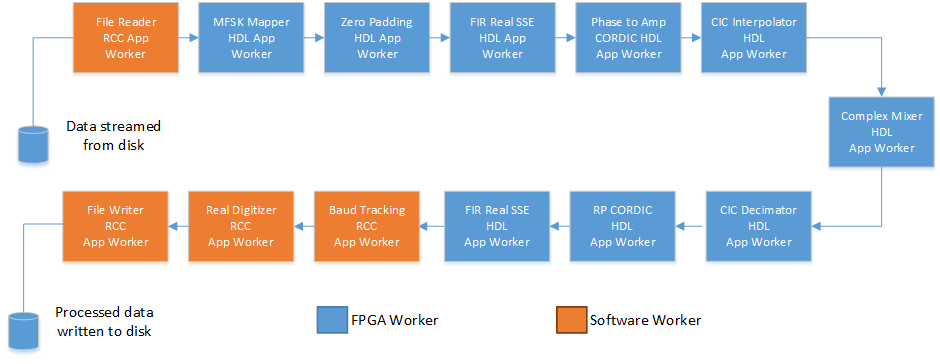
\includegraphics[scale=.65]{filerw_mode_block_diagram}
		\caption{FSK App \textit{filerw} mode Block Diagram}
		\label{fig:filerw_mode_block_diagram}
	\end{figure}
\newpage
\noindent The \textit{rx} mode inputs IQ data from the Lime ADC and processes the FSK signal down to bits that are written to file. A block diagram of the FSK App \textit{rx} mode can be seen in Figure \ref{fig:rx_mode_block_diagram}.\par\medskip
	\begin{figure}[ht]
	 	\centering
		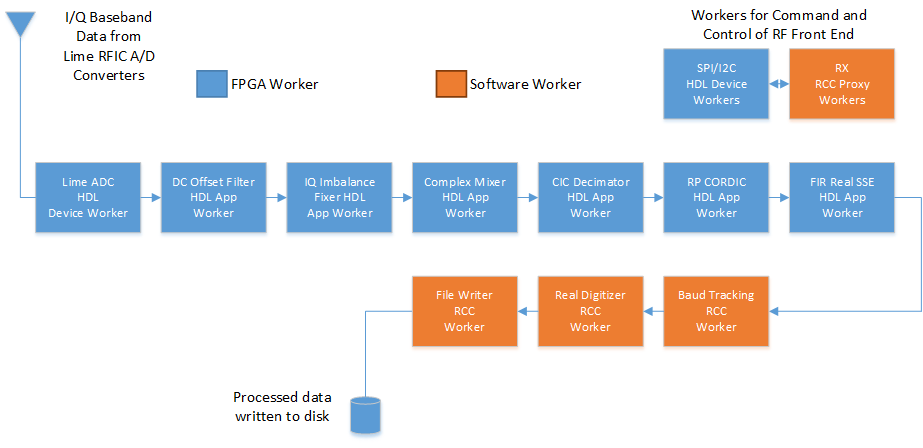
\includegraphics[scale=.65]{rx_mode_block_diagram}
		\caption{FSK App \textit{rx} mode Block Diagram}
		\label{fig:rx_mode_block_diagram}
	\end{figure}

\noindent The \textit{tx} mode inputs a file from disk, modulates the input as a FSK signal, and transmits the input via the Lime DAC. A block diagram of the FSK App \textit{tx} mode can be seen in Figure \ref{fig:tx_mode_block_diagram}.\par\medskip
	\begin{figure}[ht]
	 	\centering
		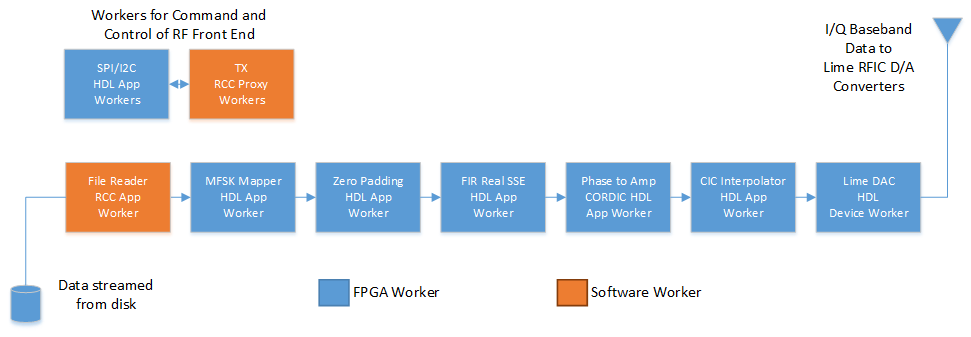
\includegraphics[scale=.65]{tx_mode_block_diagram}
		\caption{FSK App \textit{tx} mode Block Diagram}
		\label{fig:tx_mode_block_diagram}
	\end{figure}

\noindent The \textit{txrx} mode is the full transceiver mode of the application which combines the functionality of Figures \ref{fig:rx_mode_block_diagram} and \ref{fig:tx_mode_block_diagram} into a single application. This mode transmits input file data as the radio RF TX output and inputs RF RX radio input that is written to file. The \textit{bbloopback} mode utilizes the same HDL assembly and application XML as the \textit{txrx} mode but utilizes a built-in test mode of the Lime transceiver to loopback analog data at baseband.\par\medskip

\section{Building the Application}
\subsection{Dependencies}
\noindent The tables below breakdown the workers used within the various platforms and modes of the FSK App. Appendix A shows the exact worker configurations used in the HDL assemblies. See the individual component data sheets for more information and build instructions. Similarly, the HDL platform worker and configurations for the intended radio must be compiled prior to building the various FSK bitstreams.
\subsection{FSK Mode Configurations}
\subsubsection{Common to all Hardware}
	\begin{tabular}{|c|c|c|c|c|c|}
	\hline
	\rowcolor{blue}
	Application XML & filerw & rx & tx & txrx & bbloopback \\
	\hline
	app\_fsk\_filerw (dependency only, no build required) & x & • & • & • & • \\
	\rowcolor{blue}
	HDL Assemblies & filerw & rx & tx & txrx & bbloopback \\
	\hline
	fsk\_filerw & x & • & • & • & • \\
	\hline
	dc\_offset\_iq\_imbalance\_mixer\_cic\_dec\_rp\_cordic\_fir\_real & • & x & • & • & • \\
	\hline
	mfsk2\_zp16\_fir\_real\_phase\_to\_amp\_cordic\_cic\_int & • & • & x & • & • \\
	\hline
	fsk\_modem & • & • & • & x & x \\
	\hline
	\rowcolor{blue}
	RX Path Workers & filerw & rx & tx & txrx & bbloopback \\
	\hline
	dc\_offset\_filter.hdl & • & x & • & x & x \\
	\hline
	iq\_imbalance\_fixer.hdl & • & x & • & x & x \\
	\hline
	complex\_mixer.hdl & x & x & • & x & x \\
	\hline
	cic\_dec.hdl & x & x & • & x & x \\
	\hline
	rp\_cordic.hdl & x & x & • & x & x \\
	\hline
	fir\_real\_sse.hdl & x & x & • & x & x \\
	\hline
	baudTracking.rcc & x & x & • & x & x \\
	\hline
	real\_digitizer.rcc & x & x & • & x & x \\
	\hline
	file\_write.rcc & x & x & • & x & x \\
	\hline
	\rowcolor{blue}
	TX Path Workers & filerw & rx & tx & txrx & bbloopback \\
	\hline
	file\_read.rcc & x & • & x & x & x \\
	\hline
	mfsk\_mapper.hdl & x & • & x & x & x \\
	\hline
	zero\_pad.hdl & x & • & x & x & x \\
	\hline
	fir\_real\_sse.hdl & x & • & x & x & x \\
	\hline
	phase\_to\_amp\_cordic.hdl & x & • & x & x & x \\
	\hline
	cic\_int.hdl & x & • & x & x & x \\
	\hline
	\end{tabular}

\subsubsection{Additional Dependencies for Ettus E310}
	\begin{tabular}{|c|c|c|c|c|c|}
	\hline
	\rowcolor{blue}
	Application XML & filerw & rx & tx & txrx & bbloopback \\
	\hline
	app\_fsk\_rx\_e3xx (dependency only, no build required) & • & x & • & • & • \\
	\hline
	app\_fsk\_tx\_e3xx (dependency only, no build required) & • & • & x & • & • \\
	\hline
	app\_fsk\_txrx\_e3xx (dependency only, no build required) & • & •  & • & x & • \\
	\hline
	\rowcolor{blue}
	RX or TX Path Workers & filerw & rx & tx & txrx & bbloopback \\
	\hline
	ad9361\_data\_sub.hdl & • & x & x & x & • \\
	\rowcolor{blue}
	RX Path Workers & filerw & rx & tx & txrx & bbloopback \\
	\hline
	ad9361\_adc.hdl & • & x & • & x & • \\
	\hline
	ad9361\_adc\_sub.hdl & • & x & • & x & • \\
	\hline
	\rowcolor{blue}
	TX Path Workers & filerw & rx & tx & txrx & bbloopback \\
	\hline
	ad9361\_dac.hdl & • & • & x & x & • \\
	\hline
	ad9361\_dac\_sub.hdl & • & • & x & x & • \\
	\rowcolor{blue}
	Endpoint Proxies & filerw & rx & tx & txrx & bbloopback \\
	\hline
	e3xx\_rx.rcc & • & x & • & x & • \\
	\hline
	e3xx\_tx.rcc & • & • & x & x & • \\
	\hline
	\rowcolor{blue}
	SPI Command and Control & filerw & rx & tx & txrx & bbloopback \\
	\hline
	ad9361\_config.hdl & • & x & x & x & • \\
	\hline
	ad9361\_config\_proxy.rcc & • & x & x & x & •  \\
	\hline
	ad9361\_spi.hdl & • & x & x & x &   \\
	\hline
	e3xx\_mimo\_xcvr\_ad5662.hdl & • & x & x & x &   \\
	\hline
	\rowcolor{blue}
	I2C Command and Control & filerw & rx & tx & txrx & bbloopback \\
	\hline
	e3xx\_i2c.hdl & • & x & x & x &   \\
	\hline
	\rowcolor{blue}
	Analog Filter Control & filerw & rx & tx & txrx & bbloopback \\
	\hline
	e3xx\_mimo\_xcvr\_filter.hdl & • & x & x & x &   \\
	\hline
	e3xx\_mimo\_xcvr\_filter\_proxy.rcc & • & x & x & x &   \\
	\hline
	\end{tabular}

\subsubsection{Additional Dependencies for FMCOMMS2}
	\begin{tabular}{|c|c|c|c|c|c|}
	\hline
	\rowcolor{blue}
	Application XML & filerw & rx & tx & txrx & bbloopback \\
	\hline
	app\_fsk\_rx\_fmcomms2 (dependency only, no build required) & • & x & • & • & • \\
	\hline
	app\_fsk\_tx\_fmcomms2 (dependency only, no build required) & • & • & x & • & • \\
	\hline
	app\_fsk\_txrx\_fmcomms2 (dependency only, no build required) & • & •  & • & x & • \\
	\hline
	\rowcolor{blue}
	RX or TX Path Workers & filerw & rx & tx & txrx & bbloopback \\
	\hline
	ad9361\_data\_sub.hdl & • & x & x & x & • \\
	\rowcolor{blue}
	RX Path Workers & filerw & rx & tx & txrx & bbloopback \\
	\hline
	ad9361\_adc.hdl & • & x & • & x & • \\
	\hline
	ad9361\_adc\_sub.hdl & • & x & • & x & • \\
	\hline
	\rowcolor{blue}
	TX Path Workers & filerw & rx & tx & txrx & bbloopback \\
	\hline
	ad9361\_dac.hdl & • & • & x & x & • \\
	\hline
	ad9361\_dac\_sub.hdl & • & • & x & x & • \\
	\rowcolor{blue}
	Endpoint Proxies & filerw & rx & tx & txrx & bbloopback \\
	\hline
	fmcomms\_2\_3\_rx.rcc & • & x & • & x & • \\
	\hline
	fmcomms\_2\_3\_tx.rcc & • & • & x & x & • \\
	\hline
	\rowcolor{blue}
	SPI Command and Control & filerw & rx & tx & txrx & bbloopback \\
	\hline
	ad9361\_config.hdl & • & x & x & x & • \\
	\hline
	ad9361\_config\_proxy.rcc & • & x & x & x & •  \\
	\hline
	ad9361\_spi.hdl & • & x & x & x &   \\
	\hline
	\rowcolor{blue}
	I2C Command and Control & filerw & rx & tx & txrx & bbloopback \\
	\hline
	fmcomms\_2\_3\_i2c.hdl & • & x & x & x &   \\
	\hline
	\end{tabular}

\subsubsection{Additional Dependencies for FMCOMMS3}
	\begin{tabular}{|c|c|c|c|c|c|}
	\hline
	\rowcolor{blue}
	Application XML & filerw & rx & tx & txrx & bbloopback \\
	\hline
	app\_fsk\_rx\_fmcomms3 (dependency only, no build required) & • & x & • & • & • \\
	\hline
	app\_fsk\_tx\_fmcomms3 (dependency only, no build required) & • & • & x & • & • \\
	\hline
	app\_fsk\_txrx\_fmcomms3 (dependency only, no build required) & • & •  & • & x & • \\
	\hline
	\rowcolor{blue}
	RX or TX Path Workers & filerw & rx & tx & txrx & bbloopback \\
	\hline
	ad9361\_data\_sub.hdl & • & x & x & x & • \\
	\rowcolor{blue}
	RX Path Workers & filerw & rx & tx & txrx & bbloopback \\
	\hline
	ad9361\_adc.hdl & • & x & • & x & • \\
	\hline
	ad9361\_adc\_sub.hdl & • & x & • & x & • \\
	\hline
	\rowcolor{blue}
	TX Path Workers & filerw & rx & tx & txrx & bbloopback \\
	\hline
	ad9361\_dac.hdl & • & • & x & x & • \\
	\hline
	ad9361\_dac\_sub.hdl & • & • & x & x & • \\
	\rowcolor{blue}
	Endpoint Proxies & filerw & rx & tx & txrx & bbloopback \\
	\hline
	fmcomms\_2\_3\_rx.rcc & • & x & • & x & • \\
	\hline
	fmcomms\_2\_3\_tx.rcc & • & • & x & x & • \\
	\hline
	\rowcolor{blue}
	SPI Command and Control & filerw & rx & tx & txrx & bbloopback \\
	\hline
	ad9361\_config.hdl & • & x & x & x & • \\
	\hline
	ad9361\_config\_proxy.rcc & • & x & x & x & •  \\
	\hline
	ad9361\_spi.hdl & • & x & x & x &   \\
	\hline
	\rowcolor{blue}
	I2C Command and Control & filerw & rx & tx & txrx & bbloopback \\
	\hline
	fmcomms\_2\_3\_i2c.hdl & • & x & x & x &   \\
	\hline
	\end{tabular}





\subsubsection{Additional Dependencies for Matchstiq-Z1}
	\begin{tabular}{|c|c|c|c|c|c|}
	\hline
	\rowcolor{blue}
	Application XML & filerw & rx & tx & txrx & bbloopback \\
	\hline
	app\_fsk\_rx\_matchstiq\_z1 (dependency only, no build required) & • & x & • & • & • \\
	\hline
	app\_fsk\_tx\_matchstiq\_z1 (dependency only, no build required) & • & • & x & • & • \\
	\hline
	app\_fsk\_txrx\_matchstiq\_z1 (dependency only, no build required) & • & • & • & x & x \\
	\hline
	\rowcolor{blue}
	RX Path Workers & filerw & rx & tx & txrx & bbloopback \\
	\hline
	lime\_adc.hdl & • & x & • & x & x \\
	\hline
	\rowcolor{blue}
	TX Path Workers & filerw & rx & tx & txrx & bbloopback \\
	\hline
	lime\_dac.hdl & • & • & x & x & x \\
	\hline
	\rowcolor{blue}
	Endpoint Proxies & filerw & rx & tx & txrx & bbloopback \\
	\hline
	matchstiq\_z1\_rx.rcc & • & x & • & x & x \\
	\hline
	matchstiq\_z1\_tx.rcc & • & • & x & x & x \\
	\hline
	\rowcolor{blue}
	SPI Command and Control & filerw & rx & tx & txrx & bbloopback \\
	\hline
	lime\_rx\_proxy.rcc & • & x & • & x & x \\
	\hline
	lime\_rx.hdl & • & x & • & x & x \\
	\hline
	lime\_tx\_proxy.rcc & • & • & x & x & x \\
	\hline
	lime\_tx.hdl & • & • & x & x & x \\
	\hline
	lime\_spi.hdl & • & x & x & x & x \\
	\hline
	\rowcolor{blue}
	I2C Command and Control & filerw & rx & tx & txrx & bbloopback \\
	\hline
	si5338\_proxy.rcc & • & x & x & x & x \\
	\hline
	si5338.hdl & • & x & x & x & x \\
	\hline
	matchstiq\_z1\_avr\_proxy.rcc & • & x & x & x & x \\
	\hline
	matchstiq\_z1\_avr.hdl & • & x & x & x & x \\
	\hline
	tmp100\_proxy.rcc & • & x & x & x & x \\
	\hline
	tmp100.hdl & • & x & x & x & x \\
	\hline
	matchstiq\_z1\_pca9535\_proxy.rcc & • & x & x & x & x \\
	\hline
	pca9535.hdl & • & x & x & x & x \\
	\hline
	matchstiq\_z1\_i2c.hdl & • & x & x & x & x \\
	\hline
	\end{tabular}

\subsection{Additional Dependencies for Zipper-related platforms (Zedboard, Stratix IV, ML605)}
	\begin{tabular}{|c|c|c|c|c|c|}
	\hline
	\rowcolor{blue}
	Application XML & filerw & rx & tx & txrx & bbloopback \\
	\hline
	app\_fsk\_rx\_zipper (dependency only, no build required) & • & x & • & • & • \\
	\hline
	app\_fsk\_tx\_zipper (dependency only, no build required) & • & • & x & • & • \\
	\hline
	app\_fsk\_txrx\_zipper (dependency only, no build required) & • & • & • & x & x \\
	\hline
	\rowcolor{blue}
	RX Path Workers & filerw & rx & tx & txrx & bbloopback \\
	\hline
	lime\_adc.hdl & • & x & • & x & x \\
	\hline
	\rowcolor{blue}
	TX Path Workers & filerw & rx & tx & txrx & bbloopback \\
	\hline
	lime\_dac.hdl & • & • & x & x & x \\
	\hline
	\rowcolor{blue}
	Endpoint Proxies & filerw & rx & tx & txrx & bbloopback \\
	\hline
	zipper\_rx.rcc & • & x & • & x & x \\
	\hline
	zipper\_tx.rcc & • & • & x & x & x \\
	\hline
	\rowcolor{blue}
	SPI Command and Control & filerw & rx & tx & txrx & bbloopback \\
	\hline
	lime\_rx\_proxy.rcc & • & x & • & x & x \\
	\hline
	lime\_rx.hdl & • & x & • & x & x \\
	\hline
	lime\_tx\_proxy.rcc & • & • & x & x & x \\
	\hline
	lime\_tx.hdl & • & • & x & x & x \\
	\hline
	lime\_spi.hdl & • & x & x & x & x \\
	\hline
	\rowcolor{blue}
	I2C Command and Control & filerw & rx & tx & txrx & bbloopback \\
	\hline
	si5351\_proxy.rcc & • & x & x & x & x \\
	\hline
	si5351.hdl & • & x & x & x & x \\
	\hline
	\end{tabular}

	\newpage
\subsection{HDL Assembly and HDL Container}
\noindent The FPGA portion of the application consists of an HDL assembly and the HDL container. The \textit{filerw} mode uses the fsk\_filerw HDL assembly and the appropriate E310/Matchstiq-Z1/Zed-Zipper/Stratix IV/ML605 HDL container. The \textit{rx} mode uses the dc\_offset\_iq\_imbalance\_mixer\_\-cic\_dec\_rp\_cordic\_fir\_real HDL assembly and the appropriate HDL container. The \textit{tx} mode uses the mfsk2\_zp16\_fir\_real\_phase\_to\_amp\_cordic\_cic\_int HDL assembly and the appropriate HDL container. Finally, both \textit{txrx} and \textit{bbloopback} modes use the fsk\_modem HDL assembly and the appropriate HDL container. In each case the HDL assembly instances the signal processing workers while the HDL container connects those workers to the ADC and/or DAC hardware for receiving/transmitting IQ data and to the processor for reading/writing data from/to disk. The HDL container also instances command and control HDL workers required to configure the RF front end.
\subsection{Performance and Resource Utilization}
\begin{scriptsize}
\subsubsection{filerw}
%%%%%%%%%%%%%%%%%%%%%%%%%%%%%%%%%%%%%%%%%%%%%%%%%%%%%%%%%%%%
% Utilization Report for Worker "fsk_filerw"
%%%%%%%%%%%%%%%%%%%%%%%%%%%%%%%%%%%%%%%%%%%%%%%%%%%%%%%%%%%%
\begin{tabular}{|c|c|c|c|P{1.3cm}|P{1cm}|P{1.8cm}|c|}
	\hline
	\rowcolor{blue}
	Platform               & Tool    & Version & Device           & Registers (typ) & LUTs (typ)   & Control Plane Clock Fmax (MHz) (typ) & Memory/Special Functions \\
        \hline
        alst4         & Quartus & 15.1.0  & EP4SGX230KF40C2                                 & 72701     & 51,421 & 125        & \begin{tabular}{@{}c@{}}GXB Receiver PCSs=4 \\ GXB Transmitter PCSs=4 \\ GXB Transmitter PMAs=4 \\ GXB Receiver PMAs=4 \\ DSP18x18s=284 \\ PLLs=1\end{tabular} \\
        \hline
        e3xx          & Vivado  & 2017.1  & xc7z020clg484-1                                 & 24312     & 20685  & 100.000    & \begin{tabular}{@{}c@{}}BUFGs=1 \\ DSP48E1s=139 \\ RAMB36E1s=34 \\ BUFGCTRLs=1\end{tabular} \\
        \hline
        matchstiq\_z1 & Vivado  & 2017.1  & xc7z020clg484-1                                 & 24350     & 20624  & 100.000    & \begin{tabular}{@{}c@{}}BUFGs=1 \\ DSP48E1s=139 \\ RAMB36E1s=34 \\ BUFGCTRLs=1\end{tabular} \\
        \hline
        ml605         & ISE     & 14.7    & 6vlx240tff1156-1                                & 29,638    & 39,946 & 116.428    & \begin{tabular}{@{}c@{}}DSP48E1s=144 \\ RAMB36E1s=29 \\ BUFG/BUFGCTRLs=6 \\ RAMB18E1s=1\end{tabular} \\
        \hline
        zed           & Vivado  & 2017.1  & xc7z020clg484-1                                 & 23987     & 20431  & 100.000    & \begin{tabular}{@{}c@{}}BUFGs=1 \\ DSP48E1s=139 \\ RAMB36E1s=34 \\ BUFGCTRLs=1\end{tabular} \\
        \hline
        zed\_ise      & ISE     & 14.7    & 7z020clg484-1                                   & 19,264    & 25,450 & 100.080    & \begin{tabular}{@{}c@{}}DSP48E1s=144 \\ RAMB36E1s=34 \\ BUFG/BUFGCTRLs=1\end{tabular} \\
        \hline
\end{tabular}\\
\subsubsection{tx}
\begin{tabular}{|c|c|c|c|P{1.3cm}|P{1cm}|P{1.8cm}|c|}
	\hline
	\rowcolor{blue}
	Platform               & Tool    & Version & Device           & Registers (typ) & LUTs (typ)   & Control Plane Clock Fmax (MHz) (typ) & Memory/Special Functions \\
	\hline
	alst4/Zipper HSMC(A/B) & Quartus & 15.1.0  & EP4SGX230KF40C2  & 45491     & 31,434 & 125        & \begin{tabular}{@{}c@{}}GXB Receiver PCSs=4 \\ GXB Transmitter PCSs=4 \\ GXB Transmitter PMAs=4 \\ GXB Receiver PMAs=4 \\ DSP18x18s=136 \\ PLLs=1\end{tabular} \\
	\hline
	e3xx                   & Vivado  & 2017.1  & xc7z020clg484-1  & 13576     & 10899  & 100.000    & \begin{tabular}{@{}c@{}}BUFGs=2 \\ DSP48E1s=66 \\ RAMB36E1s=18 \\ BUFGCTRLs=2\end{tabular} \\
	\hline
	matchstiq\_z1          & Vivado  & 2017.1  & xc7z020clg484-1  & 13733     & 11428  & 100.000    & \begin{tabular}{@{}c@{}}BUFGs=2 \\ DSP48E1s=66 \\ RAMB36E1s=18 \\ BUFGCTRLs=2\end{tabular} \\
	\hline
	%ml605/FMCOMMS2/3 HPC   & ISE     & 14.7    & 6vlx240tff1156-1 & 13,973    & 18,223 & 125.518    & \begin{tabular}{@{}c@{}}DSP48E1s=15 \\ RAMB36E1s=18 \\ BUFG/BUFGCTRLs=6 \end{tabular} \\
	%\hline
	ml605/FMCOMMS2/3 LPC   & ISE     & 14.7    & 6vlx240tff1156-1 & 17,329    & 22,361 & 125.141    & \begin{tabular}{@{}c@{}}DSP48E1s=68 \\ RAMB36E1s=21 \\ RAMB18E1s=1 \\ BUFG/BUFGCTRLs=6 \end{tabular} \\
	\hline
	ml605/Zipper HPC       & ISE     & 14.7    & 6vlx240tff1156-1 & 17,280    & 22,422 & 125.172    & \begin{tabular}{@{}c@{}}DSP48E1s=68 \\ RAMB36E1s=21 \\ BUFG/BUFGCTRLs=7 \end{tabular} \\
	\hline
	ml605/Zipper LPC       & ISE     & 14.7    & 6vlx240tff1156-1 & 17,280    & 22,407 & 125.282    & \begin{tabular}{@{}c@{}}DSP48E1s=68 \\ RAMB36E1s=21 \\ BUFG/BUFGCTRLs=7 \end{tabular} \\
	\hline
	zed/FMCOMMS2/3         & Vivado  & 2017.1  & xc7z020clg484-1  & 12839     & 10451  & 100.000    & \begin{tabular}{@{}c@{}}BUFGs=1 \\ DSP48E1s=66 \\ RAMB36E1s=18 \\ BUFGCTRLs=1\end{tabular} \\
	\hline
	zed/Zipper             & Vivado  & 2017.1  & xc7z020clg484-1  & 12797     & 10527  & 100.000    & \begin{tabular}{@{}c@{}}BUFGs=2 \\ DSP48E1s=66 \\ RAMB36E1s=18 \\ BUFGCTRLs=2\end{tabular} \\
	\hline
	zed\_ise/FMCOMMS2/3    & ISE     & 14.7    & 7z020clg484-1    & 10,431    & 10,431 & 100.341    & \begin{tabular}{@{}c@{}}DSP48E1s=68 \\ RAMB36E1s=18 \\ BUFG/BUFGCTRLs=1\end{tabular} \\
	\hline
	zed\_ise/Zipper        & ISE     & 14.7    & 7z020clg484-1    & 10,384    & 13,506 & 100.220    & \begin{tabular}{@{}c@{}}DSP48E1s=68 \\ RAMB36E1s=18 \\ BUFG/BUFGCTRLs=2\end{tabular} \\
	\hline
\end{tabular}\\
\subsubsection{rx}
\begin{tabular}{|c|c|c|c|P{1.3cm}|P{1cm}|P{1.8cm}|c|}
	\hline
	\rowcolor{blue}
	Platform               & Tool    & Version & Device           & Registers (typ) & LUTs (typ)   & Control Plane Clock Fmax (MHz) (typ) & Memory/Special Functions \\
	\hline
	alst4/Zipper HSMC(A/B) & Quartus & 15.1.0  & EP4SGX230KF40C2  & 47752     & 34,788 & 125        & \begin{tabular}{@{}c@{}}GXB Receiver PCSs=4 \\ GXB Transmitter PCSs=4 \\ GXB Transmitter PMAs=4 \\ GXB Receiver PMAs=4 \\ DSP18x18s=166 \\ PLLs=1\end{tabular} \\
	\hline
	e3xx                   & Vivado  & 2017.1  & xc7z020clg484-1  & 15747     & 11428  & 100.000    & \begin{tabular}{@{}c@{}}BUFGs=2 \\ DSP48E1s=82 \\ RAMB36E1s=18 \\ BUFGCTRLs=2\end{tabular} \\
	\hline
	matchstiq\_z1          & Vivado  & 2017.1  & xc7z020clg484-1  & 16468     & 15747  & 100.000    & \begin{tabular}{@{}c@{}}BUFGs=2 \\ DSP48E1s=82 \\ RAMB36E1s=21 \\ BUFGCTRLs=2\end{tabular} \\
	\hline
	ml605/FMCOMMS2/3 HPC   & ISE     & 14.7    & 6vlx240tff1156-1 & 19,604    & 25,605 & 125.360    & \begin{tabular}{@{}c@{}}DSP48E1s=85 \\ RAMB36E1s=18 \\ BUFG/BUFGCTRLs=6 \end{tabular} \\
	\hline
	ml605/FMCOMMS2/3 LPC   & ISE     & 14.7    & 6vlx240tff1156-1 & 19,602    & 25,738 & 125.141    & \begin{tabular}{@{}c@{}}DSP48E1s=85 \\ RAMB36E1s=18 \\ BUFG/BUFGCTRLs=6 \end{tabular} \\
	\hline
	ml605/Zipper HPC       & ISE     & 14.7    & 6vlx240tff1156-1 & 19,482    & 25,728 &  96.600    & \begin{tabular}{@{}c@{}}DSP48E1s=85 \\ RAMB36E1s=21 \\ BUFG/BUFGCTRLs=7 \end{tabular} \\
	\hline
	ml605/Zipper LPC       & ISE     & 14.7    & 6vlx240tff1156-1 & 19,482    & 25,664 & 125.063    & \begin{tabular}{@{}c@{}}DSP48E1s=85 \\ RAMB36E1s=21 \\ BUFG/BUFGCTRLs=7 \end{tabular} \\
	\hline
	zed/FMCOMMS2/3         & Vivado  & 2017.1  & xc7z020clg484-1  & 15536     & 14682  & 100.000    & \begin{tabular}{@{}c@{}}BUFGs=1 \\ DSP48E1s=82 \\ RAMB36E1s=18 \\ BUFGCTRLs=1\end{tabular} \\
	\hline
	zed/Zipper             & Vivado  & 2017.1  & xc7z020clg484-1  & 15413     & 14660  & 100.000    & \begin{tabular}{@{}c@{}}BUFGs=2 \\ DSP48E1s=82 \\ RAMB36E1s=21 \\ BUFGCTRLs=2\end{tabular} \\
	\hline
	zed\_ise/FMCOMMS2/3    & ISE     & 14.7    & 7z020clg484-1    & 13,111    & 17,716 & 100.140    & \begin{tabular}{@{}c@{}}DSP48E1s=85 \\ RAMB36E1s=18 \\ BUFG/BUFGCTRLs=1\end{tabular} \\
	\hline
	zed\_ise/Zipper        & ISE     & 14.7    & 7z020clg484-1    & 12,990    & 17,772 & 100.462    & \begin{tabular}{@{}c@{}}DSP48E1s=85 \\ RAMB36E1s=21 \\ BUFG/BUFGCTRLs=2\end{tabular} \\
	\hline
\end{tabular}\\
\subsubsection{txrx/bbloopback}
\begin{tabular}{|c|c|c|c|P{1.3cm}|P{1cm}|P{1.8cm}|c|}
	\hline
	\rowcolor{blue}
	Platform               & Tool    & Version & Device           & Registers (typ) & LUTs (typ)   & Control Plane Clock Fmax (MHz) (typ) & Memory/Special Functions \\
	\hline
	alst4/Zipper HSMC(A/B) & Quartus & 15.1.0  & EP4SGX230KF40C2  & 75287     & 55,021 & 125        & \begin{tabular}{@{}c@{}}GXB Receiver PCSs=4 \\ GXB Transmitter PCSs=4 \\ GXB Transmitter PMAs=4 \\ GXB Receiver PMAs=4 \\ DSP18x18s=302 \\ PLLs=1\end{tabular} \\
	\hline
	e3xx                   & Vivado  & 2017.1  & xc7z020clg484-1  & 27101     & 23503  & 100.000    & \begin{tabular}{@{}c@{}}BUFGs=1 \\ DSP48E1s=148 \\ RAMB36E1s=34 \\ BUFGCTRLs=1\end{tabular} \\
	\hline
	matchstiq\_z1          & Vivado  & 2017.1  & xc7z020clg484-1  & 27371     & 24079  & 100.000    & \begin{tabular}{@{}c@{}}BUFGs=3 \\ DSP48E1s=148 \\ RAMB36E1s=37 \\ BUFGCTRLs=3\end{tabular} \\
	\hline
	%ml605/FMCOMMS2/3 HPC   & ISE     & 14.7    & 6vlx240tff1156-1 & 32,042    & 42,905 & 125.094    & \begin{tabular}{@{}c@{}}DSP48E1s=153 \\ RAMB36E1s=29 \\ BUFG/BUFGCTRLs=6 \\ RAMB18E1s=1\end{tabular} \\
	%\hline
	ml605/FMCOMMS2/3 LPC   & ISE     & 14.7    & 6vlx240tff1156-1 & 32,042    & 42,905 & 125.094    & \begin{tabular}{@{}c@{}}DSP48E1s=153 \\ RAMB36E1s=29 \\ BUFG/BUFGCTRLs=6 \\ RAMB18E1s=1\end{tabular} \\
	\hline
	ml605/Zipper HPC       & ISE     & 14.7    & 6vlx240tff1156-1 & 31,955    & 43,033 & 122.055    & \begin{tabular}{@{}c@{}}DSP48E1s=153 \\ RAMB36E1s=32 \\ BUFG/BUFGCTRLs=8 \\ RAMB18E1s=1\end{tabular} \\
	\hline
	ml605/Zipper LPC       & ISE     & 14.7    & 6vlx240tff1156-1 & 31,972    & 43,393 & 106.293    & \begin{tabular}{@{}c@{}}DSP48E1s=153 \\ RAMB36E1s=32 \\ BUFG/BUFGCTRLs=8 \\ RAMB18E1s=1\end{tabular} \\
	\hline
	zed/FMCOMMS2/3         & Vivado  & 2017.1  & xc7z020clg484-1  & 26394     & 22973  & 125.000    & \begin{tabular}{@{}c@{}}BUFGs=1 \\ DSP48E1s=148 \\ RAMB36E1s=34 \\ BUFGCTRLs=1\end{tabular} \\
	\hline
	zed/Zipper             & Vivado  & 2017.1  & xc7z020clg484-1  & 26318     & 23054  & 100.000    & \begin{tabular}{@{}c@{}}BUFGs=3 \\ DSP48E1s=148 \\ RAMB36E1s=37 \\ BUFGCTRLs=3\end{tabular} \\
	\hline
	zed\_ise/FMCOMMS2/3    & ISE     & 14.7    & 7z020clg484-1    & 21,649    & 28,536 & 100.231    & \begin{tabular}{@{}c@{}}DSP48E1s=153 \\ RAMB36E1s=34 \\ BUFG/BUFGCTRLs=1\end{tabular} \\
	\hline
	zed\_ise/Zipper        & ISE     & 14.7    & 7z020clg484-1    & 21,569    & 28,625 & 100.241    & \begin{tabular}{@{}c@{}}DSP48E1s=153 \\ RAMB36E1s=37 \\ BUFG/BUFGCTRLs=3\end{tabular} \\
	\hline
\end{tabular}\\
\end{scriptsize}
\subsection{Executable}
The software portion of the application consists of a C++ program written using the OpenCPI C++ API as well as RCC proxy workers for command and control functionality. The program references the appropriate application XML file for the requested hardware and mode. The app XML files contain all of the property settings for the components in each application, except for the configuration of the endpoint proxy(ies). These endpoint proxy-related settings are passed via command-line prompted values to the appropriate endpoint proxy workers.\\
To build for the host platform (which is the case if ML605 or Stratix IV platform is intended to be used), run the following commands from the FSK directory:\par\medskip
\texttt{ ocpidev build}\par\medskip
\noindent To build for the Zedboard or Matchstiq-Z1 (which run the xilinx13\_3 PetaLinux operating system), run the following command from the FSK directory:\par\medskip 
\texttt{ ocpidev build --rcc-platform xilinx13\_3 }\par\medskip
\noindent To build for the Ettus E310 (which runs the xilinx13\_4 PetaLinux operating system), run the following command from the FSK directory:\par\medskip 
\texttt{ ocpidev build --rcc-platform xilinx13\_4 }\par\medskip
Note that the Ettus E310 BSP project contains its own updated copy of the FSK app that should be used.

\section{Testing the Application}
\subsection{Baud Synchronization}
The input filename for the application is idata/Os.jpeg. It is modified from an original JPEG image (see Figure \ref{fig:os_pic}) with data prepended to it for baud synchronization purposes (240 bytes of an alternating 1-0 pattern followed by 2 bytes are the value 0xFACE). In the receive data stream, real\_digitizer.rcc worker makes symbol/bit decisions and only sends out bits that occur after the first detecteed 0xFACE bit pattern (b1111101011001110).
\subsection{Sample test setup}
The test setup varies per mode of operation. The base test setup includes a hardware platform of choice and appropriate power and USB cables (E310, Matchstiq-Z1 and Zedboard/Zipper use the USB cable to access the terminal via a program such as \textit{screen} or over a USB-over-Ethernet connection; Stratix IV and ML605 require a USB cable for JTAG loading). All other test modes expand upon this base configuration, and may or may not include additional RF cabling or external equipment.\par\medskip
\noindent The \textit{filerw} mode requires only the base test setup since no transceiver operations are actuated (data passes to and from the FPGA in a ``loopback'' fashion). Upon application execution, the expected result is written to odata/out\_app\_fsk\_filerw.bin, which is a transmitted copy of the input file idata/Os.jpeg.\par\medskip
\noindent The \textit{bbloopback} mode is similar to the \textit{filerw} mode, but data goes beyond the FPGA through the radio's built-in analog baseband loopback, and back into the FPGA. Because the data never reaches the TX/RX connectors, no external RF cabling is required. The expected result is a transmitted copy of the idata/Os.jpeg file as the output odata/out\_app\_fsk\_bbloopback.bin.\par\medskip
\noindent The next mode is the \textit{rx} mode, which requires the base test setup with an RX antenna, as well as another transmitter (such as another platform running the \textit{tx} mode) in order to broadcast a known FSK signal. Optionally, a spectrum analyzer may be connected to the transmitter to visually verify that the signal being fed into the radio's RX input is an FSK signal at the correct RF frequency and bandwidth. The output is written to the file odata/out\_app\_fsk\_rx.bin.\par\medskip
\noindent The next mode is the \textit{tx} mode, which requires the base test setup with a TX antenna, as well as some hardware to verify the transmission, such as a spectrum analyzer or an additional radio running in \textit{rx} mode. In this mode the input file idata/Os.jpeg is transmitted out of the RF TX output of the radio.\par\medskip
\noindent The final mode is the \textit{txrx} mode. This mode requires a base test setup with either a SMA loopback cable connecting the TX output of the radio to the RX input of the radio, or separate RX/TX antennas if RF usage is desired. An RF splitter can also be used to optionally connect a spectrum analyzer to the RF signal for visual verification. The default values for RF gain assume that an RF splitter is being used.\par\medskip
\subsection{make show}
In order to test the application using the various modes mentioned above, \texttt{make show} can be run from the \texttt{applications/FSK} directory. This provides instructions (for Zynq-Based Platforms) for setting \texttt{OCPI\_LIBRARY\_PATH} on the hardware platform and then running the application. Finally, it explains how to verify the output data on the development computer. The following sections provide further insight into these instructions.
\subsection{Artifacts}
Before running the application, the location of the required deployable artifacts must be specified in the \texttt{OCPI\_LIBRARY\_PATH} environment variable. Separate artifacts are needed for each RCC worker, and one artifact for the required FPGA image. Furthermore, artifacts differ depending on which mode the application is to be run in. Appendix B includes a list of the artifacts required for each platform and mode.
\subsection{Arguments to executable}
There is only one required initial argument to the FSK App executable, which defines the mode of execution. There is an optional initial argument to the FSK App executable that defines whether or not to run in debug mode. The app prompts the user at runtime for additional values, which vary depending upon the selected mode of operation. Running the application without any arguments prints the usage instructions. The non-initial optional arguments prompt the user to override the default value(s), and primarily configure the RF front end of the given platform using one or more endpoint proxies.\par\medskip
\noindent The arguments to the executable are summarized in the following table:\\
\begin{tabular}{|l|l|l|}
\hline
\rowcolor{blue}
Argument & Mode & Description \\
\hline
mode & n/a & filerw, rx, tx, txrx, bbloopback\\
\hline
debug\_mode & optional - `d' or blank & enables initial and final dump of all properties\\
\hline
\end{tabular}\par\medskip
\noindent The prompts performed by the executable are summarized in the following table:\\
\begin{tabular}{|l|l|l|}
\hline
\rowcolor{blue}
Argument & Mode & Description \\
\hline
RF frontend (ML605 and zed only) & rx, txrx & zipper, FMCOMMS2, or FMCOMMS3\\
\hline
runtime & filerw, rx, tx, txrx, bbloopback & run time of application in seconds\\
\hline
rx\_sample\_rate & rx, txrx, bbloopback & RX RF sample rate in Msps\\
\hline
rx\_rf\_center\_freq & rx, txrx, bbloopback & RX RF tuning frequency in MHz\\
\hline
rx\_rf\_bw & rx, txrx, bbloopback & RX RF bandwidth in MHz\\
\hline
rx\_rf\_gain & rx, txrx, bbloopback & RX RF gain in dB\\
\hline
rx\_bb\_bw & rx, txrx, bbloopback & RX baseband bandwidth in MHz\\
\hline
rx\_bb\_gain & rx, txrx, bbloopback & RX baseband gain in dB\\
\hline
rx\_if\_center\_freq & rx, txrx, bbloopback & RX IF tuning frequency in MHz. 0 disables IF tuning\\
\hline
tx\_sample\_rate & tx, txrx, bbloopback & TX RF sample rate in Msps\\
\hline
tx\_rf\_center\_freq & tx, txrx, bbloopback & TX RF tuning frequency in MHz\\
\hline
tx\_rf\_gain & tx, txrx, bbloopback & TX RF gain in dB\\
\hline
tx\_bb\_bw & tx, txrx, bbloopback & TX baseband bandwidth in MHz\\
\hline
tx\_bb\_gain & tx, txrx, bbloopback & TX baseband gain in dB\\
\hline
\end{tabular}\par\medskip\medskip

\noindent Example arguments for the \textbf{Ettus E310 BSP} using the SMA ports RX=RX2A TX=TRXA:\\
\begin{tabular}{|l|l|}
\hline
\rowcolor{blue}
Parameter 	&        Value  	\\
\hline
RF frontend 	&        (not set / default)  	\\
\hline
Runtime (s) 	&        20 	        \\
\hline
RX SMA channel 	&        RX2A              	\\
\hline
TX SMA channel 	&        TRXA           	\\
\hline
rx\_sample\_rate 	&4 	                \\
\hline
rx\_rf\_center\_freq 	&3000  	\\
\hline
rx\_rf\_bw 	&        -1 (default)   \\
\hline
rx\_rf\_gain 	&        12       	\\
\hline
rx\_bb\_bw 	&        4 	        \\
\hline
rx\_bb\_gain 	&        -1 (default) 	\\
\hline
rx\_if\_center\_freq 	&0              	\\
\hline
tx\_sample\_rate 	&4              	\\
\hline
tx\_rf\_center\_freq 	&3000 	        \\
\hline
tx\_rf\_bw 	&        -1 (default)   \\
\hline
tx\_rf\_gain 	&        -28 	        \\
\hline
tx\_bb\_bw 	&        4        	\\
\hline
tx\_bb\_gain    &       -1 (default) \\
\hline
\end{tabular}\par\medskip

\noindent Note that if the application complains about the output file or directory, run `\code{mkdir odata}' in the FSK directory and rerun the executable.
\pagebreak
\subsection{Library Path Requirements}
\noindent Prior to running the application, the environment variable OCPI\_LIBRARY\_PATH must include the following directories:\par\medskip
	\begin{itemize}
		\item ocpi.core component RCC library location
		\item ocpi.assets bitstream directory location
		\item ocpi.assets.devices library location
		\item ocpi.assets component RCC library location
	\end{itemize}
Ettus E310 additionally requires the following:
	\begin{itemize}
		\item ocpi.bsp.e310 bitstream directory location
		\item ocpi.bsp.e310.devices library location
		\item ocpi.bsp.e310.cards library location
	\end{itemize}
Matchstiq-Z1 additionally requires the following:
	\begin{itemize}
		\item ocpi.assets.platforms.matchstiq\_z1.devices library location
	\end{itemize}

\noindent Note that the Stratix IV GX230 and ML605 hardware setups require the intended slot-specific bitstream's file location to be first in OCPI\_LIBRARY\_PATH. This is necessary because ocpirun's aritifact compatibility test does not currently differentiate between slot-connected device workers for multiple bitstreams that contain the same device worker, in the scenario where what differentiates the bitstreams is the device worker's slot connectivity. Reference the OpenCPI Application Development Guide for more about OCPI\_LIBRARY\_PATH. \par\medskip

\noindent Examples of library paths that could be used can be seen below:\\

Note: All example paths are relative to the applications/FSK/ directory.\\

\noindent\textbf{Recommended Library Path for Ettus E310}\\
%%OCPI_LIBRARY_PATH=$OCPI_PROJECT_REGISTRY_DIR/ocpi.core/exports/lib:$OCPI_PROJECT_REGISTRY_DIR/ocpi.assets/exports/lib
\verb|OCPI_LIBRARY_PATH=$OCPI_CDK_DIR/../projects/core/exports/lib:\| \\
\verb|<path-to-mounted-assets-project>/exports/lib:\| \\
\verb|<path-to-mounted-e310-bsp--project>/exports/lib| \\

\noindent\textbf{Recommended Library Path for Matchstiq-Z1 or Zedboard or ML605/FMCOMMS2/3-HPC}\\
%%OCPI_LIBRARY_PATH=$OCPI_PROJECT_REGISTRY_DIR/ocpi.core/exports/lib:$OCPI_PROJECT_REGISTRY_DIR/ocpi.assets/exports/lib
\verb|OCPI_LIBRARY_PATH=$OCPI_PROJECT_REGISTRY_DIR/ocpi.core/exports/lib:$OCPI_PROJECT\| \\
\verb|_REGISTRY_DIR/ocpi.assets/exports/lib| \\

\noindent\textbf{Recommended Library Path \textit{filerw} mode}\\
%%OCPI_LIBRARY_PATH=$OCPI_PROJECT_REGISTRY_DIR/ocpi.core/exports/lib:$OCPI_PROJECT_REGISTRY_DIR/ocpi.assets/exports/lib
\verb|OCPI_LIBRARY_PATH=$OCPI_PROJECT_REGISTRY_DIR/ocpi.core/exports/lib:$OCPI_PROJECT\| \\
\verb|_REGISTRY_DIR/ocpi.assets/exports/lib| \\

\noindent\textbf{Recommended Library Path for Stratix IV GX230/Zipper in HSMC A}\\
\noindent\textbf{\textit{rx}}\\
%\verb|OCPI_LIBRARY_PATH=$PWD/../../hdl/assemblies/dc_offset_iq_imbalance_mixer_cic_dec_rp_cordic_fir_real|\\
%OCPI_LIBRARY_PATH=$OCPI_PROJECT_REGISTRY_DIR/ocpi.core/exports/lib:$OCPI_PROJECT_REGISTRY_DIR/ocpi.assets/exports/lib:../../hdl/assemblies/dc_offset_iq_imbalance_mixer_cic_dec_timestamper/container-dc_offset_iq_imbalance_mixer_cic_dec_timestamper_alst4_alst4_zipper_hsmc_alst4_port_a_rx_cnt_1rx_0tx_thruasm_zipper_hsmc_a_alst4/
\verb|OCPI_LIBRARY_PATH=$OCPI_PROJECT_REGISTRY_DIR/ocpi.core/exports/lib:$OCPI_PROJECT\| \\
\verb|_REGISTRY_DIR/ocpi.assets/exports/lib:../../hdl/assemblies/dc_offset_iq_imbalanc\| \\
\verb|e_mixer_cic_dec_rp_cordic_fir_real/container-dc_offset_iq_imbalance_mixer_cic_de\| \\
\verb|c_rp_cordic_fir_real_alst4_alst4_zipper_hsmc_alst4_port_a_rx_cnt_1rx_0tx_thruasm\| \\
\verb|_zipper_hsmc_a_alst4/| \\

\noindent\textbf{\textit{tx}}\\
%OCPI_LIBRARY_PATH=$OCPI_PROJECT_REGISTRY_DIR/ocpi.core/exports/lib/:$OCPI_PROJECT_REGISTRY_DIR/ocpi.assets/exports/lib/:../../hdl/assemblies/mfsk2_zp16_fir_real_phase_to_amp_cordic_cic_int/container-mfsk2_zp16_fir_real_phase_to_amp_cordic_cic_int_alst4_alst4_zipper_hsmc_alst4_port_a_tx_cnt_0rx_1tx_thruasm_zipper_hsmc_a_alst4/
\verb|OCPI_LIBRARY_PATH=$OCPI_PROJECT_REGISTRY_DIR/ocpi.core/exports/lib/:$OCPI_PROJEC\| \\
\verb|T_REGISTRY_DIR/ocpi.assets/exports/lib/:../../hdl/assemblies/mfsk2_zp16_fir_real\| \\
\verb|_phase_to_amp_cordic_cic_int/container-mfsk2_zp16_fir_real_phase_to_amp_cordic_c\| \\
\verb|ic_int_alst4_alst4_zipper_hsmc_alst4_port_a_tx_cnt_0rx_1tx_thruasm_zipper_hsmc_a\| \\
\verb|_alst4/| \\

\noindent\textbf{\textit{txrx/bbloopback}}\\
%OCPI_LIBRARY_PATH=$OCPI_PROJECT_REGISTRY_DIR/ocpi.core/exports/lib/:$OCPI_PROJECT_REGISTRY_DIR/ocpi.assets/exports/lib/:../../hdl/assemblies/fsk_modem/container-fsk_modem_alst4_alst4_zipper_hsmc_alst4_port_a_rx_tx_cnt_1rx_1tx_thruasm_zipper_hsmc_a_alst4/
\verb|OCPI_LIBRARY_PATH=$OCPI_PROJECT_REGISTRY_DIR/ocpi.core/exports/lib/:$OCPI_PROJEC\| \\
\verb|T_REGISTRY_DIR/ocpi.assets/exports/lib/:../../hdl/assemblies/fsk_modem/container\| \\
\verb|-fsk_modem_alst4_alst4_zipper_hsmc_alst4_port_a_rx_tx_cnt_1rx_1tx_thruasm_zipper\| \\
\verb|_hsmc_a_alst4/| \\
\par\medskip

\noindent\textbf{Recommended Library Path for Stratix IV GX230/Zipper in HSMC B}\\

\noindent\textbf{\textit{rx}}\\
%OCPI_LIBRARY_PATH=$OCPI_PROJECT_REGISTRY_DIR/ocpi.core/exports/lib:$OCPI_PROJECT_REGISTRY_DIR/ocpi.assets/exports/lib:../../hdl/assemblies/dc_offset_iq_imbalance_mixer_cic_dec_timestamper/container-dc_offset_iq_imbalance_mixer_cic_dec_timestamper_alst4_alst4_zipper_hsmc_alst4_port_b_rx_cnt_1rx_0tx_thruasm_zipper_hsmc_b_alst4/
\verb|OCPI_LIBRARY_PATH=$OCPI_PROJECT_REGISTRY_DIR/ocpi.core/exports/lib:$OCPI_PROJECT\| \\
\verb|_REGISTRY_DIR/ocpi.assets/exports/lib:../../hdl/assemblies/dc_offset_iq_imbalanc\| \\
\verb|e_mixer_cic_dec_rp_cordic_fir_real/container-dc_offset_iq_imbalance_mixer_cic_de\| \\
\verb|c_rp_cordic_fir_real_alst4_alst4_zipper_hsmc_alst4_port_b_rx_cnt_1rx_0tx_thruasm\| \\
\verb|_zipper_hsmc_b_alst4/| \\

\noindent\textbf{\textit{tx}}\\
%OCPI_LIBRARY_PATH=$OCPI_PROJECT_REGISTRY_DIR/ocpi.core/exports/lib/:$OCPI_PROJECT_REGISTRY_DIR/ocpi.assets/exports/lib/:../../hdl/assemblies/mfsk2_zp16_fir_real_phase_to_amp_cordic_cic_int/container-mfsk2_zp16_fir_real_phase_to_amp_cordic_cic_int_alst4_alst4_zipper_hsmc_alst4_port_b_tx_cnt_0rx_1tx_thruasm_zipper_hsmc_b_alst4/
\verb|OCPI_LIBRARY_PATH=$OCPI_PROJECT_REGISTRY_DIR/ocpi.core/exports/lib/:$OCPI_PROJEC\| \\
\verb|T_REGISTRY_DIR/ocpi.assets/exports/lib/:../../hdl/assemblies/mfsk2_zp16_fir_real\| \\
\verb|_phase_to_amp_cordic_cic_int/container-mfsk2_zp16_fir_real_phase_to_amp_cordic_c\| \\
\verb|ic_int_alst4_alst4_zipper_hsmc_alst4_port_b_tx_cnt_0rx_1tx_thruasm_zipper_hsmc_b\| \\
\verb|_alst4/| \\

\noindent\textbf{\textit{txrx/bbloopback}}\\
%OCPI_LIBRARY_PATH=$OCPI_PROJECT_REGISTRY_DIR/ocpi.core/exports/lib/:$OCPI_PROJECT_REGISTRY_DIR/ocpi.assets/exports/lib/:../../hdl/assemblies/fsk_modem/container-fsk_modem_alst4_alst4_zipper_hsmc_alst4_port_b_rx_tx_cnt_1rx_1tx_thruasm_zipper_hsmc_b_alst4/
\verb|OCPI_LIBRARY_PATH=$OCPI_PROJECT_REGISTRY_DIR/ocpi.core/exports/lib/:$OCPI_PROJEC\| \\
\verb|T_REGISTRY_DIR/ocpi.assets/exports/lib/:../../hdl/assemblies/fsk_modem/container\| \\
\verb|-fsk_modem_alst4_alst4_zipper_hsmc_alst4_port_b_rx_tx_cnt_1rx_1tx_thruasm_zipper\| \\
\verb|_hsmc_b_alst4/| \\
\par\medskip
\pagebreak

\noindent\textbf{Recommended Library Path for ML605/Zipper in FMC LPC}\\

\noindent\textbf{\textit{rx}}\\
%OCPI_LIBRARY_PATH=$OCPI_PROJECT_REGISTRY_DIR/ocpi.core/exports/lib:$OCPI_PROJECT_REGISTRY_DIR/ocpi.assets/exports/lib:../../hdl/assemblies/dc_offset_iq_imbalance_mixer_cic_dec_timestamper/container-dc_offset_iq_imbalance_mixer_cic_dec_timestamper_ml605_ml605_zipper_fmc_lpc_rx_cnt_1rx_0tx_thruasm_zipper_lpc_ml605/
\verb|OCPI_LIBRARY_PATH=$OCPI_PROJECT_REGISTRY_DIR/ocpi.core/exports/lib:$OCPI_PROJECT\| \\
\verb|_REGISTRY_DIR/ocpi.assets/exports/lib:../../hdl/assemblies/dc_offset_iq_imbalanc\| \\
\verb|e_mixer_cic_dec_rp_cordoc_fir_real/container-dc_offset_iq_imbalance_mixer_cic_de\| \\
\verb|c_rp_cordic_fir_real_ml605_ml605_zipper_fmc_lpc_rx_cnt_1rx_0tx_thruasm_zipper_lp\| \\
\verb|c_ml605/|\\


\noindent\textbf{\textit{tx}}\\
%OCPI_LIBRARY_PATH=$OCPI_PROJECT_REGISTRY_DIR/ocpi.core/exports/lib/:$OCPI_PROJECT_REGISTRY_DIR/ocpi.assets/exports/lib/:../../hdl/assemblies/mfsk2_zp16_fir_real_phase_to_amp_cordic_cic_int/container-mfsk2_zp16_fir_real_phase_to_amp_cordic_cic_int_ml605_ml605_zipper_fmc_lpc_tx_cnt_0rx_1tx_thruasm_zipper_lpc_ml605/
\verb|OCPI_LIBRARY_PATH=$OCPI_PROJECT_REGISTRY_DIR/ocpi.core/exports/lib/:$OCPI_PROJEC\| \\
\verb|T_REGISTRY_DIR/ocpi.assets/exports/lib/:../../hdl/assemblies/mfsk2_zp16_fir_real\| \\
\verb|_phase_to_amp_cordic_cic_int/container-mfsk2_zp16_fir_real_phase_to_amp_cordic_c\| \\
\verb|ic_int_ml605_ml605_zipper_fmc_lpc_tx_cnt_0rx_1tx_thruasm_zipper_lpc_ml605/| \\

\noindent\textbf{\textit{txrx/bbloopback}}\\
%OCPI_LIBRARY_PATH=$OCPI_PROJECT_REGISTRY_DIR/ocpi.core/exports/lib/:$OCPI_PROJECT_REGISTRY_DIR/ocpi.assets/exports/lib/:../../hdl/assemblies/fsk_modem/container-fsk_modem_ml605_ml605_zipper_fmc_lpc_rx_tx_cnt_1rx_1tx_thruasm_zipper_lpc_ml605/
\verb|OCPI_LIBRARY_PATH=$OCPI_PROJECT_REGISTRY_DIR/ocpi.core/exports/lib/:$OCPI_PROJEC\| \\
\verb|T_REGISTRY_DIR/ocpi.assets/exports/lib/:../../hdl/assemblies/fsk_modem/container\| \\
\verb|-fsk_modem_ml605_ml605_zipper_fmc_lpc_rx_tx_cnt_1rx_1tx_thruasm_zipper_lpc_ml605\| \\
\verb|/| \\
\par\medskip

\noindent\textbf{Example ML605/Zipper in FMC HPC}\\
\noindent\textbf{\textit{rx}}\\
%OCPI_LIBRARY_PATH=$OCPI_PROJECT_REGISTRY_DIR/ocpi.core/exports/lib:$OCPI_PROJECT_REGISTRY_DIR/ocpi.assets/exports/lib:../../hdl/assemblies/dc_offset_iq_imbalance_mixer_cic_dec_timestamper/container-dc_offset_iq_imbalance_mixer_cic_dec_timestamper_ml605_ml605_zipper_fmc_hpc_rx_cnt_1rx_0tx_thruasm_zipper_hpc_ml605/
\verb|OCPI_LIBRARY_PATH=$OCPI_PROJECT_REGISTRY_DIR/ocpi.core/exports/lib:$OCPI_PROJECT\| \\
\verb|_REGISTRY_DIR/ocpi.assets/exports/lib:../../hdl/assemblies/dc_offset_iq_imbalanc\| \\
\verb|e_mixer_cic_dec_rp_cordic_fir_real/container-dc_offset_iq_imbalance_mixer_cic_de\| \\
\verb|c_rp_cordic_fir_real_ml605_ml605_zipper_fmc_hpc_rx_cnt_1rx_0tx_thruasm_zipper_hp\| \\
\verb|c_ml605/| \\

\noindent\textbf{\textit{tx}}\\
%OCPI_LIBRARY_PATH=$OCPI_PROJECT_REGISTRY_DIR/ocpi.core/exports/lib/:$OCPI_PROJECT_REGISTRY_DIR/ocpi.assets/exports/lib/:../../hdl/assemblies/mfsk2_zp16_fir_real_phase_to_amp_cordic_cic_int/container-mfsk2_zp16_fir_real_phase_to_amp_cordic_cic_int_ml605_ml605_zipper_fmc_hpc_tx_cnt_0rx_1tx_thruasm_zipper_hpc_ml605/
\verb|OCPI_LIBRARY_PATH=$OCPI_PROJECT_REGISTRY_DIR/ocpi.core/exports/lib/:$OCPI_PROJEC\| \\
\verb|T_REGISTRY_DIR/ocpi.assets/exports/lib/:../../hdl/assemblies/mfsk2_zp16_fir_real\| \\
\verb|_phase_to_amp_cordic_cic_int/container-mfsk2_zp16_fir_real_phase_to_amp_cordic_c\| \\
\verb|ic_int_ml605_ml605_zipper_fmc_hpc_tx_cnt_0rx_1tx_thruasm_zipper_hpc_ml605/| \\

\noindent\textbf{\textit{txrx/bbloopback}}\\
%OCPI_LIBRARY_PATH=$OCPI_PROJECT_REGISTRY_DIR/ocpi.core/exports/lib/:$OCPI_PROJECT_REGISTRY_DIR/ocpi.assets/exports/lib/:../../hdl/assemblies/fsk_modem/container-fsk_modem_ml605_ml605_zipper_fmc_hpc_rx_tx_cnt_1rx_1tx_thruasm_zipper_hpc_ml605/
\verb|OCPI_LIBRARY_PATH=$OCPI_PROJECT_REGISTRY_DIR/ocpi.core/exports/lib/:$OCPI_PROJEC\| \\
\verb|T_REGISTRY_DIR/ocpi.assets/exports/lib/:../../hdl/assemblies/fsk_modem/container\| \\
\verb|-fsk_modem_ml605_ml605_zipper_fmc_hpc_rx_tx_cnt_1rx_1tx_thruasm_zipper_hpc_ml605/| \\
\pagebreak

\subsection{Expected results}
\noindent In the case of the \textit{filerw}, \textit{rx}, \textit{txrx}, and \textit{bbloopback} modes, assuming transmission of the idata/Os.jpeg input file, the expected result is a transmitted copy of the JPEG file. A Linux program such as Eye of GNOME (eog) may be used to display the JPEG file. The file is shown in Figure \ref{fig:os_pic}.\par\medskip
\noindent In the case of the \textit{tx} mode, verification is obtained by viewing the RF spectrum on a spectrum analyzer. An example of the transmitted spectrum may be seen in Figure \ref{fig:tx_spec_an}.\par\medskip
	\begin{figure}[ht]
	 	\centering
	 	\begin{minipage}{.325\textwidth}
			\centering\includegraphics[width=1.0\linewidth]{Os}
			\caption{FSK input file}
			\label{fig:os_pic}
		\end{minipage}
	 	\begin{minipage}{.45\textwidth}
			\centering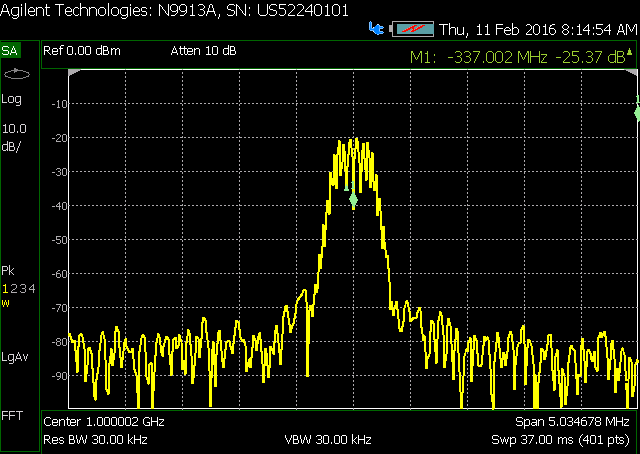
\includegraphics[width=1.0\linewidth]{tx_spec_an}
			\caption{Output of FSK App RF transmit}
			\label{fig:tx_spec_an}
		\end{minipage}
	\end{figure}
\pagebreak
\subsection{Known Issues}
\noindent
\begin{itemize}
  \item The \textit{rx} and \textit{tx} modes suffer from limited carrier recovery ability. The requested center frequency may need to be adjusted to a value other than the exact expected nominal value.
  \item For more information on known limitations when using the Zipper-related platforms (Zedboard, Stratix IV, ML605), see the document Myriad-RF\_1\_Zipper\_Limitations included with this project.
  \item  On x86 host machines with more than one Stratix IV and/or ML605s plugged into PCIe slots, this app will assume that the first found Stratix IV/ML605 has a Zipper/MyriadRF plugged in. The first found Stratix IV/ML605 will be used during execution. While there are means to address this issue, they have not been implemented for the current release.
  \item Sometimes the radio can get into an unwanted state. If unusual results are seen, run \code{ocpihdl unload} and rerun the application.
\end{itemize}

\pagebreak
\section{Appendix A: Worker Parameters}
Configuration information for each component in the application can be found in the application XML for that configuration. \textit{E.g.} for the Ettus E310 in txrx mode, \code{app\_fsk\_txrx\_e3xx}. Further information can be determined by browsing the chosen platform configurations and container XMLs for the given configuration and platform.
\section{Appendix B: Artifacts}
Each worker that is required for a given configuration of this application has an artifact that must be found at runtime (located via one of the \code{OCPI\_LIBRARAY\_PATH} choices listed above). Reference the lists of workers for each configuration and platform to determine the artifacts required. Each required RCC worker corresponds to a required \\
\code{target-<shortened-rcc-platform>/<worker>\_s.so} artifact. All required HDL workers (together) correspond to a single required \code{<assembly>\_<platform>\_<platform-config>\_<container>.bitz} artifact.\\
\subsection{Ettus E310}
	\noindent\textbf{filerw}
	\begin{itemize}
	\begin{minipage}[t]{.5\textwidth}
	\item fsk\_filerw\_e3xx\_base.bitz

	\item target-linux-x13\_4-arm/file\_read\_s.so
	\item target-linux-x13\_4-arm/Baudtracking\_simple\_s.so
	\end{minipage}
	\begin{minipage}[t]{.5\textwidth}
	\item target-linux-x13\_4-arm/real\_digitizer\_s.so
	\item target-linux-x13\_4-arm/file\_write\_s.so
	\end{minipage}
	\end{itemize}

	\noindent\textbf{rx}
	\begin{itemize}
  \item dc\_offset\_iq\_imbalance\_mixer\_cic\_dec\_rp\_cordic\_fir\_real\_e3xx\_cfg\_1rx\_0tx\_mode\_2\_cmos\_cnt\_1rx\_0tx\_mode\_2\_ \\
	bypassasm\_e3xx\_mimo\_xcvr\_CMOS\_e3xx.bitz \\

	\begin{minipage}[t]{.5\textwidth}
	\item target-linux-x13\_4-arm/Baudtracking\_simple\_s.so
	\item target-linux-x13\_4-arm/real\_digitizer\_s.so
	\item target-linux-x13\_4-arm/file\_write\_s.so
	\end{minipage}
	\begin{minipage}[t]{.5\textwidth}
	\item target-linux-x13\_4-arm/ad9361\_config\_proxy\_s.so
	\item target-linux-x13\_4-arm/e3xx\_mimo\_xcvr\_filter\_proxy\_s.so
	\item target-linux-x13\_4-arm/e3xx\_rx\_s.so
	\end{minipage}
	\end{itemize}

	\noindent\textbf{tx}
	\begin{itemize}
  \item mfsk2\_zp16\_fir\_real\_phase\_to\_amp\_cordic\_cic\_int\_e3xx\_cfg\_0rx\_1tx\_mode\_2\_cmos\_cnt\_0rx\_1tx\_mode\_2\_thruasm\_ \\
	e3xx\_mimo\_xcvr\_CMOS\_e3xx.bitz \\

	\begin{minipage}[t]{.5\textwidth}
	\item target-linux-x13\_4-arm/file\_read\_s.so
	\item target-linux-x13\_4-arm/ad9361\_config\_proxy\_s.so
	\end{minipage}
	\begin{minipage}[t]{.5\textwidth}
	\item target-linux-x13\_4-arm/e3xx\_mimo\_xcvr\_filter\_proxy\_s.so
	\item target-linux-x13\_4-arm/e3xx\_tx\_s.so
	\end{minipage}
	\end{itemize}

	\noindent\textbf{txrx/bbloopback}
	\begin{itemize}
  \item fsk\_modem\_e3xx\_cfg\_1rx\_1tx\_mode\_2\_cmos\_cnt\_1rx\_1tx\_mode\_2\_thruasm\_e3xx\_mimo\_xcvr\_CMOS\_e3xx.bitz \\

	\begin{minipage}[t]{.5\textwidth}
	\item target-linux-x13\_4-arm/file\_read\_s.so
	\item target-linux-x13\_4-arm/Baudtracking\_simple\_s.so
	\item target-linux-x13\_4-arm/real\_digitizer\_s.so
	\end{minipage}
	\begin{minipage}[t]{.5\textwidth}
	\item target-linux-x13\_4-arm/file\_write\_s.so
	\item target-linux-x13\_4-arm/ad9361\_config\_proxy\_s.so
	\item target-linux-x13\_4-arm/e3xx\_mimo\_xcvr\_filter\_proxy\_s.so
	\item target-linux-x13\_4-arm/e3xx\_rx\_s.so
	\item target-linux-x13\_4-arm/e3xx\_tx\_s.so
	\end{minipage}
	\end{itemize}




\pagebreak
\subsection{Zedboard/FMCOMMS2/3}
	\noindent\textbf{filerw (FMCOMMS2/3 not required)}
	\begin{itemize}
	\begin{minipage}[t]{.5\textwidth}
	\item fsk\_filerw\_zed\_base.bitz
	\item target-linux-x13\_3-arm/file\_read\_s.so
	\item target-linux-x13\_3-arm/Baudtracking\_simple\_s.so
	\end{minipage}
	\begin{minipage}[t]{.5\textwidth}
	\item target-linux-x13\_3-arm/real\_digitizer\_s.so
	\item target-linux-x13\_3-arm/file\_write\_s.so
	\end{minipage}
	\end{itemize}

	\noindent\textbf{rx}
	\begin{itemize}
  \item dc\_offset\_iq\_imbalance\_mixer\_cic\_dec\_timestamper\_zed\_cfg\_1rx\_0\\
tx\_fmcomms\_2\_3\_lpc\_lvds\_cnt\_1rx\_0tx\_thruasm\_fmcomms\_2\_3\_lpc\_LVDS\_zed.bitz \\
	\begin{minipage}[t]{.5\textwidth}
	\item target-linux-x13\_3-arm/Baudtracking\_simple\_s.so
	\item target-linux-x13\_3-arm/real\_digitizer\_s.so
	\item target-linux-x13\_3-arm/file\_write\_s.so
	\end{minipage}
	\begin{minipage}[t]{.5\textwidth}
	\item target-linux-x13\_3-arm/zipper\_rx\_s.so
	\item target-linux-x13\_3-arm/lime\_rx\_proxy\_s.so
	\item target-linux-x13\_3-arm/si5351\_proxy\_s.so
	\end{minipage}
	\end{itemize}

	\noindent\textbf{tx}
	\begin{itemize}
  \item mfsk2\_zp16\_fir\_real\_phase\_to\_amp\_cordic\_cic\_int\_zed\_cfg\_0rx\_\\
1tx\_fmcomms\_2\_3\_lpc\_lvds\_cnt\_0rx\_1tx\_thruasm\_fmcomms\_2\_3\_lpc\_LVDS\_zed.bitz
\\ \\
	\begin{minipage}[t]{.5\textwidth}
	\item target-linux-x13\_3-arm/file\_read\_s.so
	\item target-linux-x13\_3-arm/zipper\_tx\_s.so
	\end{minipage}
	\begin{minipage}[t]{.5\textwidth}
	\item target-linux-x13\_3-arm/lime\_tx\_proxy\_s.so
	\item target-linux-x13\_3-arm/si5351\_proxy\_s.so
	\end{minipage}
	\end{itemize}

	\noindent\textbf{txrx/bbloopback}
	\begin{itemize}
  \item fsk\_modem\_zed\_cfg\_1rx\_1tx\_fmcomms\_2\_3\_lpc\_lvds\_cnt\_1rx\_1tx\_\\
thruasm\_fmcomms\_2\_3\_lpc\_LVDS\_zed.bitz \\
	\begin{minipage}[t]{.5\textwidth}
	\item target-linux-x13\_3-arm/file\_read\_s.so
	\item target-linux-x13\_3-arm/Baudtracking\_simple\_s.so
	\item target-linux-x13\_3-arm/real\_digitizer\_s.so
	\item target-linux-x13\_3-arm/file\_write\_s.so
	\end{minipage}
	\begin{minipage}[t]{.5\textwidth}
	\item target-linux-x13\_3-arm/zipper\_rx\_s.so
	\item target-linux-x13\_3-arm/zipper\_tx\_s.so
	\item target-linux-x13\_3-arm/lime\_rx\_proxy\_s.so
	\item target-linux-x13\_3-arm/lime\_tx\_proxy\_s.so
	\item target-linux-x13\_3-arm/si5351\_proxy\_s.so
	\end{minipage}
	\end{itemize}




\pagebreak
\subsection{Matchstiq-Z1}
	\noindent\textbf{filerw}
	\begin{itemize}
	\begin{minipage}[t]{.5\textwidth}
	\item fsk\_filerw\_matchstiq\_z1\_base.bitz
	\item target-linux-x13\_3-arm/file\_read\_s.so
	\item target-linux-x13\_3-arm/Baudtracking\_simple\_s.so
	\end{minipage}
	\begin{minipage}[t]{.5\textwidth}
	\item target-linux-x13\_3-arm/real\_digitizer\_s.so
	\item target-linux-x13\_3-arm/file\_write\_s.so
	\end{minipage}
	\end{itemize}

	\noindent\textbf{rx}
	\begin{itemize}
	\item dc\_offset\_iq\_imbalance\_mixer\_cic\_dec\_rp\_cordic\_fir\_real\_matchstiq\_z1\_matchstiq\_z1\_rx\_cnt\_1rx\_0tx\_ \\ thruasm\_matchstiq\_z1.bitz \\ \\
	\begin{minipage}[t]{.5\textwidth}\item target-linux-x13\_3-arm/Baudtracking\_simple\_s.so
	\item target-linux-x13\_3-arm/real\_digitizer\_s.so
	\item target-linux-x13\_3-arm/file\_write\_s.so
	\item target-linux-x13\_3-arm/matchstiq\_z1\_rx\_s.so
	\item target-linux-x13\_3-arm/lime\_rx\_proxy\_s.so
	\end{minipage}
	\begin{minipage}[t]{.5\textwidth}	\item target-linux-x13\_3-arm/si5338\_proxy\_s.so
	\item target-linux-x13\_3-arm/matchstiq\_z1\_avr\_proxy\_s.so
	\item target-linux-x13\_3-arm/tmp100\_proxy\_s.so
	\item target-linux-x13\_3-arm/matchstiq\_z1\_pca9535\_proxy\_s.so
	\end{minipage}
	\end{itemize}

	\noindent\textbf{tx}
	\begin{itemize}
	\item
mfsk2\_zp16\_fir\_real\_phase\_to\_amp\_cordic\_cic\_int\_matchstiq\_z1\_matchstiq\_z1\_tx\_cnt\_0rx\_1tx\_thruasm\_matchstiq\_z1.bitz	\\ \\
	\begin{minipage}[t]{.5\textwidth}
	\item target-linux-x13\_3-arm/file\_read\_s.so
	\item target-linux-x13\_3-arm/matchstiq\_z1\_tx\_s.so
	\item target-linux-x13\_3-arm/lime\_tx\_proxy\_s.so
	\item target-linux-x13\_3-arm/si5338\_proxy\_s.so
	\end{minipage}
	\begin{minipage}[t]{.5\textwidth}
	\item target-linux-x13\_3-arm/matchstiq\_z1\_avr\_proxy\_s.so
	\item target-linux-x13\_3-arm/tmp100\_proxy\_s.so
	\item target-linux-x13\_3-arm/matchstiq\_z1\_pca9535\_proxy\_s.so
	\end{minipage}
	\end{itemize}

	\noindent\textbf{txrx/bbloopback}
	\begin{itemize}
	\item fsk\_modem\_matchstiq\_z1\_matchstiq\_z1\_rx\_tx\_cnt\_1rx\_1tx\_thruasm\_matchstiq\_z1.bitz \\ \\
	\begin{minipage}[t]{.5\textwidth}
	\item target-linux-x13\_3-arm/file\_read\_s.so
	\item target-linux-x13\_3-arm/Baudtracking\_simple\_s.so
	\item target-linux-x13\_3-arm/real\_digitizer\_s.so
	\item target-linux-x13\_3-arm/file\_write\_s.so
	\item target-linux-x13\_3-arm/matchstiq\_z1\_rx\_s.so
	\item target-linux-x13\_3-arm/matchstiq\_z1\_tx\_s.so
	\end{minipage}
	\begin{minipage}[t]{.5\textwidth}
	\item target-linux-x13\_3-arm/lime\_rx\_proxy\_s.so
	\item target-linux-x13\_3-arm/lime\_tx\_proxy\_s.so
	\item target-linux-x13\_3-arm/si5338\_proxy\_s.so
	\item target-linux-x13\_3-arm/matchstiq\_z1\_avr\_proxy\_s.so
	\item target-linux-x13\_3-arm/tmp100\_proxy\_s.so
	\item target-linux-x13\_3-arm/matchstiq\_z1\_pca9535\_proxy\_s.so
	\end{minipage}
	\end{itemize}
\pagebreak
\subsection{Zedboard/Zipper}
	\noindent\textbf{filerw (zipper not required)}
	\begin{itemize}
	\begin{minipage}[t]{.5\textwidth}
	\item fsk\_filerw\_zed\_base.bitz
	\item target-linux-x13\_3-arm/file\_read\_s.so
	\item target-linux-x13\_3-arm/Baudtracking\_simple\_s.so
	\end{minipage}
	\begin{minipage}[t]{.5\textwidth}
	\item target-linux-x13\_3-arm/real\_digitizer\_s.so
	\item target-linux-x13\_3-arm/file\_write\_s.so
	\end{minipage}
	\end{itemize}

	\noindent\textbf{rx}
	\begin{itemize}
	\item dc\_offset\_iq\_imbalance\_mixer\_cic\_dec\_rp\_cordic\_fir\_real\_zed\_base\_cnt\_1rx\_0tx\_thruasm\_zipper\_lpc\_zed.bitz \\ \\
	\begin{minipage}[t]{.5\textwidth}
	\item target-linux-x13\_3-arm/Baudtracking\_simple\_s.so
	\item target-linux-x13\_3-arm/real\_digitizer\_s.so
	\item target-linux-x13\_3-arm/file\_write\_s.so
	\end{minipage}
	\begin{minipage}[t]{.5\textwidth}
	\item target-linux-x13\_3-arm/zipper\_rx\_s.so
	\item target-linux-x13\_3-arm/lime\_rx\_proxy\_s.so
	\item target-linux-x13\_3-arm/si5351\_proxy\_s.so
	\end{minipage}
	\end{itemize}

	\noindent\textbf{tx}
	\begin{itemize}
	\item mfsk2\_zp16\_fir\_real\_phase\_to\_amp\_cordic\_cic\_int\_zed\_base\_cnt\_0rx\_1tx\_thruasm\_zipper\_lpc\_zed.bitz
\\ \\
	\begin{minipage}[t]{.5\textwidth}
	\item target-linux-x13\_3-arm/file\_read\_s.so
	\item target-linux-x13\_3-arm/zipper\_tx\_s.so
	\end{minipage}
	\begin{minipage}[t]{.5\textwidth}
	\item target-linux-x13\_3-arm/lime\_tx\_proxy\_s.so
	\item target-linux-x13\_3-arm/si5351\_proxy\_s.so
	\end{minipage}
	\end{itemize}

	\noindent\textbf{txrx/bbloopback}
	\begin{itemize}
	\item fsk\_modem\_zed\_base\_cnt\_1rx\_1tx\_thruasm\_zipper\_lpc\_zed.bitz \\ \\
	\begin{minipage}[t]{.5\textwidth}
	\item target-linux-x13\_3-arm/file\_read\_s.so
	\item target-linux-x13\_3-arm/Baudtracking\_simple\_s.so
	\item target-linux-x13\_3-arm/real\_digitizer\_s.so
	\item target-linux-x13\_3-arm/file\_write\_s.so
	\end{minipage}
	\begin{minipage}[t]{.5\textwidth}
	\item target-linux-x13\_3-arm/zipper\_rx\_s.so
	\item target-linux-x13\_3-arm/zipper\_tx\_s.so
	\item target-linux-x13\_3-arm/lime\_rx\_proxy\_s.so
	\item target-linux-x13\_3-arm/lime\_tx\_proxy\_s.so
	\item target-linux-x13\_3-arm/si5351\_proxy\_s.so
	\end{minipage}
	\end{itemize}

\pagebreak
\subsection{Stratix IV/Zipper}
	\noindent\textbf{filerw (zipper not required)}
	\begin{itemize}
	\begin{minipage}[t]{.5\textwidth}
	\item fsk\_filerw\_alst4\_base.bitz
	\item target-linux-c7-x86\_64/file\_read\_s.so
	\item target-linux-c7-x86\_64/Baudtracking\_simple\_s.so
	\end{minipage}
	\begin{minipage}[t]{.5\textwidth}
	\item target-linux-c7-x86\_64/real\_digitizer\_s.so
	\item target-linux-c7-x86\_64/file\_write\_s.so
	\end{minipage}
	\end{itemize}

	\noindent\textbf{rx}
	\begin{itemize}
	\begin{minipage}[t]{.5\textwidth}
	\item target-linux-c7-x86\_64/file\_read\_s.so
	\item target-linux-c7-x86\_64/Baudtracking\_simple\_s.so
	\item target-linux-c7-x86\_64/real\_digitizer\_s.so
	\end{minipage}
	\begin{minipage}[t]{.5\textwidth}
	\item target-linux-c7-x86\_64/zipper\_rx\_s.so
	\item target-linux-c7-x86\_64/lime\_rx\_proxy\_s.so
	\item target-linux-c7-x86\_64/si5351\_proxy\_s.so
	\end{minipage}
	\end{itemize}
	For Zipper plugged into HSMC Port A:
	\begin{itemize}
	\item dc\_offset\_iq\_imbalance\_mixer\_cic\_dec\_rp\_cordic\_fir\_real\_alst4\_alst4\_zipper\_hsmc\_alst4\_port\_a\_ \\
		rx\_cnt\_1rx\_0tx\_thruasm\_zipper\_hsmc\_a\_alst4.bitz
	\end{itemize}
	For Zipper plugged into HSMC Port B:
	\begin{itemize}
	\item dc\_offset\_iq\_imbalance\_mixer\_cic\_dec\_rp\_cordic\_fir\_real\_alst4\_alst4\_zipper\_hsmc\_alst4\_port\_b\_ \\
		rx\_cnt\_1rx\_0tx\_thruasm\_zipper\_hsmc\_b\_alst4.bitz		
	\end{itemize}

	\noindent\textbf{tx}
	\begin{itemize}
	\begin{minipage}[t]{.5\textwidth}
	\item target-linux-c7-x86\_64/file\_read\_s.so
	\item target-linux-c7-x86\_64/zipper\_tx\_s.so
	\end{minipage}
	\begin{minipage}[t]{.5\textwidth}
	\item target-linux-c7-x86\_64/lime\_tx\_proxy\_s.so
	\item target-linux-c7-x86\_64/si5351\_proxy\_s.so
	\end{minipage}
	\end{itemize}
	For Zipper plugged into HSMC Port A:
	\begin{itemize}
	\item mfsk2\_zp16\_fir\_real\_phase\_to\_amp\_cordic\_cic\_int\_alst4\_alst4\_zipper\_hsmc\_alst4\_port\_a\_\\
		txcnt\_0rx\_1tx\_thruasm\_zipper\_hsmc\_a\_alst4.bitz
	\end{itemize}
	For Zipper plugged into HSMC Port B:
	\begin{itemize}
	\item mfsk2\_zp16\_fir\_real\_phase\_to\_amp\_cordic\_cic\_int\_alst4\_alst4\_zipper\_hsmc\_alst4\_port\_b\_\\
		tx\_cnt\_0rx\_1tx\_thruasm\_zipper\_hsmc\_b\_alst4.bitz 
	\end{itemize}

	\noindent\textbf{txrx/bbloopback}
	\begin{itemize}
	\begin{minipage}[t]{.5\textwidth}
	\item target-linux-c7-x86\_64/file\_read\_s.so
	\item target-linux-c7-x86\_64/Baudtracking\_simple\_s.so
	\item target-linux-c7-x86\_64/real\_digitizer\_s.so
	\item target-linux-c7-x86\_64/zipper\_rx\_s.so
	\end{minipage}
	\begin{minipage}[t]{.5\textwidth}
	\item target-linux-c7-x86\_64/zipper\_tx\_s.so
	\item target-linux-c7-x86\_64/lime\_rx\_proxy\_s.so
	\item target-linux-c7-x86\_64/lime\_tx\_proxy\_s.so
	\item target-linux-c7-x86\_64/si5351\_proxy\_s.so
	\end{minipage}
	\end{itemize}
	For Zipper plugged into HSMC Port A:
	\begin{itemize}
		\item fsk\_modem\_alst4\_alst4\_zipper\_hsmc\_alst4\_port\_a\_rx\_tx\_cnt\_1rx\_1tx\_thruasm\_zipper\_hsmc\_a\_alst4.bitz 
	\end{itemize}
	\noindent For Zipper plugged into HSMC Port B:
	\begin{itemize}
		\item fsk\_modem\_alst4\_alst4\_zipper\_hsmc\_alst4\_port\_b\_rx\_tx\_cnt\_1rx\_1tx\_thruasm\_zipper\_hsmc\_b\_alst4.bitz
	\end{itemize}





\pagebreak
\subsection{ML605/FMCOMMS2/3}
	\noindent\textbf{filerw (FMCOMMS2/3 not required)}
	\begin{itemize}
	\begin{minipage}[t]{.5\textwidth}
	\item fsk\_filerw\_ml605\_base.bitz
	\item target-linux-c7-x86\_64/file\_read\_s.so
	\item target-linux-c7-x86\_64/Baudtracking\_simple\_s.so
	\end{minipage}
	\begin{minipage}[t]{.5\textwidth}
	\item target-linux-c7-x86\_64/real\_digitizer\_s.so
	\item target-linux-c7-x86\_64/file\_write\_s.so
	\end{minipage}
	\end{itemize}
	
	\noindent\textbf{rx}
	\begin{itemize}
	\begin{minipage}[t]{.5\textwidth}
	\item target-linux-c7-x86\_64/file\_read\_s.so
	\item target-linux-c7-x86\_64/Baudtracking\_simple\_s.so
	\item target-linux-c7-x86\_64/real\_digitizer\_s.so
	\end{minipage}
	\begin{minipage}[t]{.5\textwidth}
	\item target-linux-c7-x86\_64/zipper\_rx\_s.so
	\item target-linux-c7-x86\_64/lime\_rx\_proxy\_s.so
	\item target-linux-c7-x86\_64/si5351\_proxy\_s.so
	\end{minipage}
	\end{itemize}
	\noindent For FMCOMMS2/3 plugged into FMC LPC:
	\begin{itemize}
	\item dc\_offset\_iq\_imbalance\_mixer\_cic\_dec\_timestamper\_ml605\_cfg\_1rx\_0tx \\
\_fmcomms\_2\_3\_lpc\_lvds\_cnt\_1rx\_0tx\_thruasm\_fmcomms\_2\_3\_lpc\_LVDS\_ml605.bitz
	\end{itemize}
	\noindent For FMCOMMS2/3 plugged into FMC HPC:
	\begin{itemize}
	\item dc\_offset\_iq\_imbalance\_mixer\_cic\_dec\_timestamper\_ml605\_cfg\_1rx\_0tx \\
\_fmcomms\_2\_3\_hpc\_lvds\_cnt\_1rx\_0tx\_thruasm\_fmcomms\_2\_3\_hpc\_LVDS\_ml605.bitz
	\end{itemize}
	
	\noindent\textbf{tx}
	\begin{itemize}
	\begin{minipage}[t]{.5\textwidth}
	\item target-linux-c7-x86\_64/file\_read\_s.so
	\item target-linux-c7-x86\_64/zipper\_tx\_s.so
	\end{minipage}
	\begin{minipage}[t]{.5\textwidth}
	\item target-linux-c7-x86\_64/lime\_tx\_proxy\_s.so
	\item target-linux-c7-x86\_64/si5351\_proxy\_s.so
	\end{minipage}
	\end{itemize}
	For Zipper plugged into FMC LPC:
	\begin{itemize}
		\item mfsk2\_zp16\_fir\_real\_phase\_to\_amp\_cordic\_cic\_int\_ml605\_cfg\_0rx\\
\_1tx\_fmcomms\_2\_3\_lpc\_lvds\_cnt\_0rx\_1tx\_thruasm\_fmcomms\_2\_3\_lpc\_LVDS\_ml605.bitz
	\end{itemize}

	\noindent\textbf{txrx/bbloopback}
	\begin{itemize}
	\begin{minipage}[t]{.5\textwidth}
	\item target-linux-c7-x86\_64/file\_read\_s.so
	\item target-linux-c7-x86\_64/Baudtracking\_simple\_s.so
	\item target-linux-c7-x86\_64/real\_digitizer\_s.so
	\item target-linux-c7-x86\_64/zipper\_rx\_s.so
	\end{minipage}
	\begin{minipage}[t]{.5\textwidth}
	\item target-linux-c7-x86\_64/zipper\_tx\_s.so
	\item target-linux-c7-x86\_64/lime\_rx\_proxy\_s.so
	\item target-linux-c7-x86\_64/lime\_tx\_proxy\_s.so
	\item target-linux-c7-x86\_64/si5351\_proxy\_s.so
	\end{minipage}
	\end{itemize}
	For Zipper plugged into FMC LPC:
	\begin{itemize}
		\item fsk\_modem\_ml605\_cfg\_1rx\_1tx\_fmcomms\_2\_3\_lpc\_lvds\_cnt\_1rx\_1tx\\
\_thruasm\_fmcomms\_2\_3\_lpc\_LVDS\_ml605.bitz
	\end{itemize}







\pagebreak
\subsection{ML605/Zipper}
	\noindent\textbf{filerw (zipper not required)}
	\begin{itemize}
	\begin{minipage}[t]{.5\textwidth}
	\item fsk\_filerw\_ml605\_base.bitz
	\item target-linux-c7-x86\_64/file\_read\_s.so
	\item target-linux-c7-x86\_64/Baudtracking\_simple\_s.so
	\end{minipage}
	\begin{minipage}[t]{.5\textwidth}
	\item target-linux-c7-x86\_64/real\_digitizer\_s.so
	\item target-linux-c7-x86\_64/file\_write\_s.so
	\end{minipage}
	\end{itemize}
	
	\noindent\textbf{rx}
	\begin{itemize}
	\begin{minipage}[t]{.5\textwidth}
	\item target-linux-c7-x86\_64/file\_read\_s.so
	\item target-linux-c7-x86\_64/Baudtracking\_simple\_s.so
	\item target-linux-c7-x86\_64/real\_digitizer\_s.so
	\end{minipage}
	\begin{minipage}[t]{.5\textwidth}
	\item target-linux-c7-x86\_64/zipper\_rx\_s.so
	\item target-linux-c7-x86\_64/lime\_rx\_proxy\_s.so
	\item target-linux-c7-x86\_64/si5351\_proxy\_s.so
	\end{minipage}
	\end{itemize}
	For Zipper plugged into FMC LPC:
	\begin{itemize}
	\item dc\_offset\_iq\_imbalance\_mixer\_cic\_dec\_rp\_cordic\_fir\_real\_ml605\_cfg\_1rx\_0tx\_fmcomms\_2\_3\_lpc\_ \\
	lvds\_cnt\_1rx\_0tx\_thruasm\_fmcomms\_2\_3\_lpc\_LVDS\_ml605.bitz
	\end{itemize}
	\noindent For Zipper plugged into FMC HPC:
	\begin{itemize}
	\item dc\_offset\_iq\_imbalance\_mixer\_cic\_dec\_rp\_cordic\_fir\_real\_ml605\_cfg\_1rx\_0tx\_fmcomms\_2\_3\_hpc\_ \\
	lvds\_cnt\_1rx\_0tx\_thruasm\_fmcomms\_2\_3\_hpc\_LVDS\_ml605.bitz
	\end{itemize}
	
	\noindent\textbf{tx}
	\begin{itemize}
	\begin{minipage}[t]{.5\textwidth}
	\item target-linux-c7-x86\_64/file\_read\_s.so
	\item target-linux-c7-x86\_64/zipper\_tx\_s.so
	\end{minipage}
	\begin{minipage}[t]{.5\textwidth}
	\item target-linux-c7-x86\_64/lime\_tx\_proxy\_s.so
	\item target-linux-c7-x86\_64/si5351\_proxy\_s.so
	\end{minipage}
	\end{itemize}
	For Zipper plugged into FMC LPC:
	\begin{itemize}
		\item mfsk2\_zp16\_fir\_real\_phase\_to\_amp\_cordic\_cic\_int\_ml605\_ml605\_zipper\_fmc\_lpc\_ \\
		tx\_cnt\_0rx\_1tx\_thruasm\_zipper\_lpc\_ml605.bitz
	\end{itemize}
	\noindent For Zipper plugged into FMC HPC:
	\begin{itemize}
		\item mfsk2\_zp16\_fir\_real\_phase\_to\_amp\_cordic\_cic\_int\_ml605\_ml605\_zipper\_fmc\_hpc\_ \\
		tx\_cnt\_0rx\_1tx\_thruasm\_zipper\_hpc\_ml605.bitz
	\end{itemize}

	\noindent\textbf{txrx/bbloopback}
	\begin{itemize}
	\begin{minipage}[t]{.5\textwidth}
	\item target-linux-c7-x86\_64/file\_read\_s.so
	\item target-linux-c7-x86\_64/Baudtracking\_simple\_s.so
	\item target-linux-c7-x86\_64/real\_digitizer\_s.so
	\item target-linux-c7-x86\_64/zipper\_rx\_s.so
	\end{minipage}
	\begin{minipage}[t]{.5\textwidth}
	\item target-linux-c7-x86\_64/zipper\_tx\_s.so
	\item target-linux-c7-x86\_64/lime\_rx\_proxy\_s.so
	\item target-linux-c7-x86\_64/lime\_tx\_proxy\_s.so
	\item target-linux-c7-x86\_64/si5351\_proxy\_s.so
	\end{minipage}
	\end{itemize}
	For Zipper plugged into FMC LPC:
	\begin{itemize}
		\item fsk\_modem\_ml605\_ml605\_zipper\_fmc\_hpc\_rx\_tx\_cnt\_1rx\_1tx\_thruasm\_zipper\_lpc\_ml605.bitz
	\end{itemize}
	\noindent For Zipper plugged into FMC HPC:
	\begin{itemize}
		\item fsk\_modem\_ml605\_ml605\_zipper\_fmc\_hpc\_rx\_tx\_cnt\_1rx\_1tx\_thruasm\_zipper\_hpc\_ml605.bitz
	\end{itemize}
\end{document}
